\section{Results}
We illustrate the results in three directions, hedging effectiveness,
ability of hedging extreme negative events in $r^S$, and the stability of $h^*$.

%\begin{itemize}
%   \item  Hedging Effectiveness
%   \begin{itemize}
%     \item Kick out Frank for its ineffectiveness; Alternative to a one-parameter symmetric Archimedean copula is Plackett;
       \natp{\em [The issue with the Frank copula is that is has no
         tails. A scatterplot looks like a strip, there is no
         concentration in the tails. For CDO pricing (and this is what
         I remember from my PhD studies) this poses problems as you
         move from senior to junior tranches. Here, I suppose it just
         does not capture the empirical behaviour of the data.
         ]}
%     \item Differences among combinations of copula and risk reduction objective are small;
%     \item None of the combination can escape from the structural break point (dependence of training is stronger then that of testing). (The bump in 25-26th Sept 2019)
%     \item The best performing RRO of a particular risk measure in out-of-sample $r^h$ is not necessarily same, e.g.
%      VaR 95\% as RRO (with Gumbel copula) can generate the lowest out-of-sample ES 99\%.
%   \end{itemize}
%   \item Ability to hedge extreme events in $r^S$
%   \begin{itemize}
%     \item The extreme events in $r^S$ are well managed by the hedge.
%     The magnitudes of loss in $r^h$ is much smaller than that of $r^h$. (Visually seen from the time series of $r^h$)
%     \item None of the combination can escape from the structural break point (dependence of training is stronger then that of testing)
%   \end{itemize}
%   \item Stability of $h^\ast$
%   \begin{itemize}
%     \item Gumbel gives high $h$ all the time; the extreme events are "hedged" ex-ante.
%     \item ES 99\% and VaR 99\% as risk reduction objective are too sensitive to extremes in training data;
%     Large changes in $h$ are suggested in response to extremes training data, while the testing data are less extreme;
%     \item ERM can be seen as a smoothed risk measure focusing in the lower tail of $r^h$; Less sensitive to rare events; Suggested.
%   \end{itemize}
%\item \end{itemize}


\subsection{Hedging Effectiveness}\label{subsec:hedging-effectiveness}
The hedging effectiveness (HE) is defined as
\begin{align}
  1- \frac{\rho(r^h)}{\rho(r^S)}.
  \end{align}
The hedging effectiveness is the reduction of portfolio risk.
This notion of evaluating of hedging performance was proposed by \citet{ederington1979hedging} in the context of, at that time, hedging the newly introduced
organized futures market.
\citet{ederington1979hedging}  evaluates the extent of variance reduction by introducing another asset.
We also measure the hedging effectiveness in other risk measure mentioned in section \ref{subsec:spectral-risk-measures},
e.g. via Expected Shortfall (ES)
\begin{align}
  1- \frac{\text{ES}_\alpha(r^h)}{\text{ES}_\alpha(r^S)}.
  \end{align}

The box-plots in figure \ref{fig:OOSHE} show the out-of-sample hedging effectiveness of different copulas under various risk
reduction objectives across testing datasets.
Observe that most of the copulae perform well.
The average HE of copulas and risk reduction objectives is higher than 60\% except for Frank-copula.
However, the HEs vary a lot in different testing data.
In some instances, the HE can be as low as 10\%.
This reflects the highly violate nature of cryptocurrencies:
the optimal hedge ratio in the training data deviates from that of testing data.
There is a large literature about structural break points and time changing dependence, to name a few
\citet{hafner2012dynamic}, \citet{patton2006modelling}, \citet{creal2008general},
\citet{engle2002dynamic}, \citet{giacomini2009inhomogeneous}, and also
\citet{manner2012survey}.\medskip

Frank-copula, in general, is not a good choice to model financial data.
We can see from figure~\ref{fig:Frank} that the Frank copula is not fitting the Bitcoin and its future visually, no matter
which optimization procedure is being deployed.
The samples of Frank diffuse like a strip with parallel edge when the parameter $\theta$ decrease (samples are being less dependent).
This makes Frank copula not a a good fit to the data.

\begin{figure}[th]
   \centering
   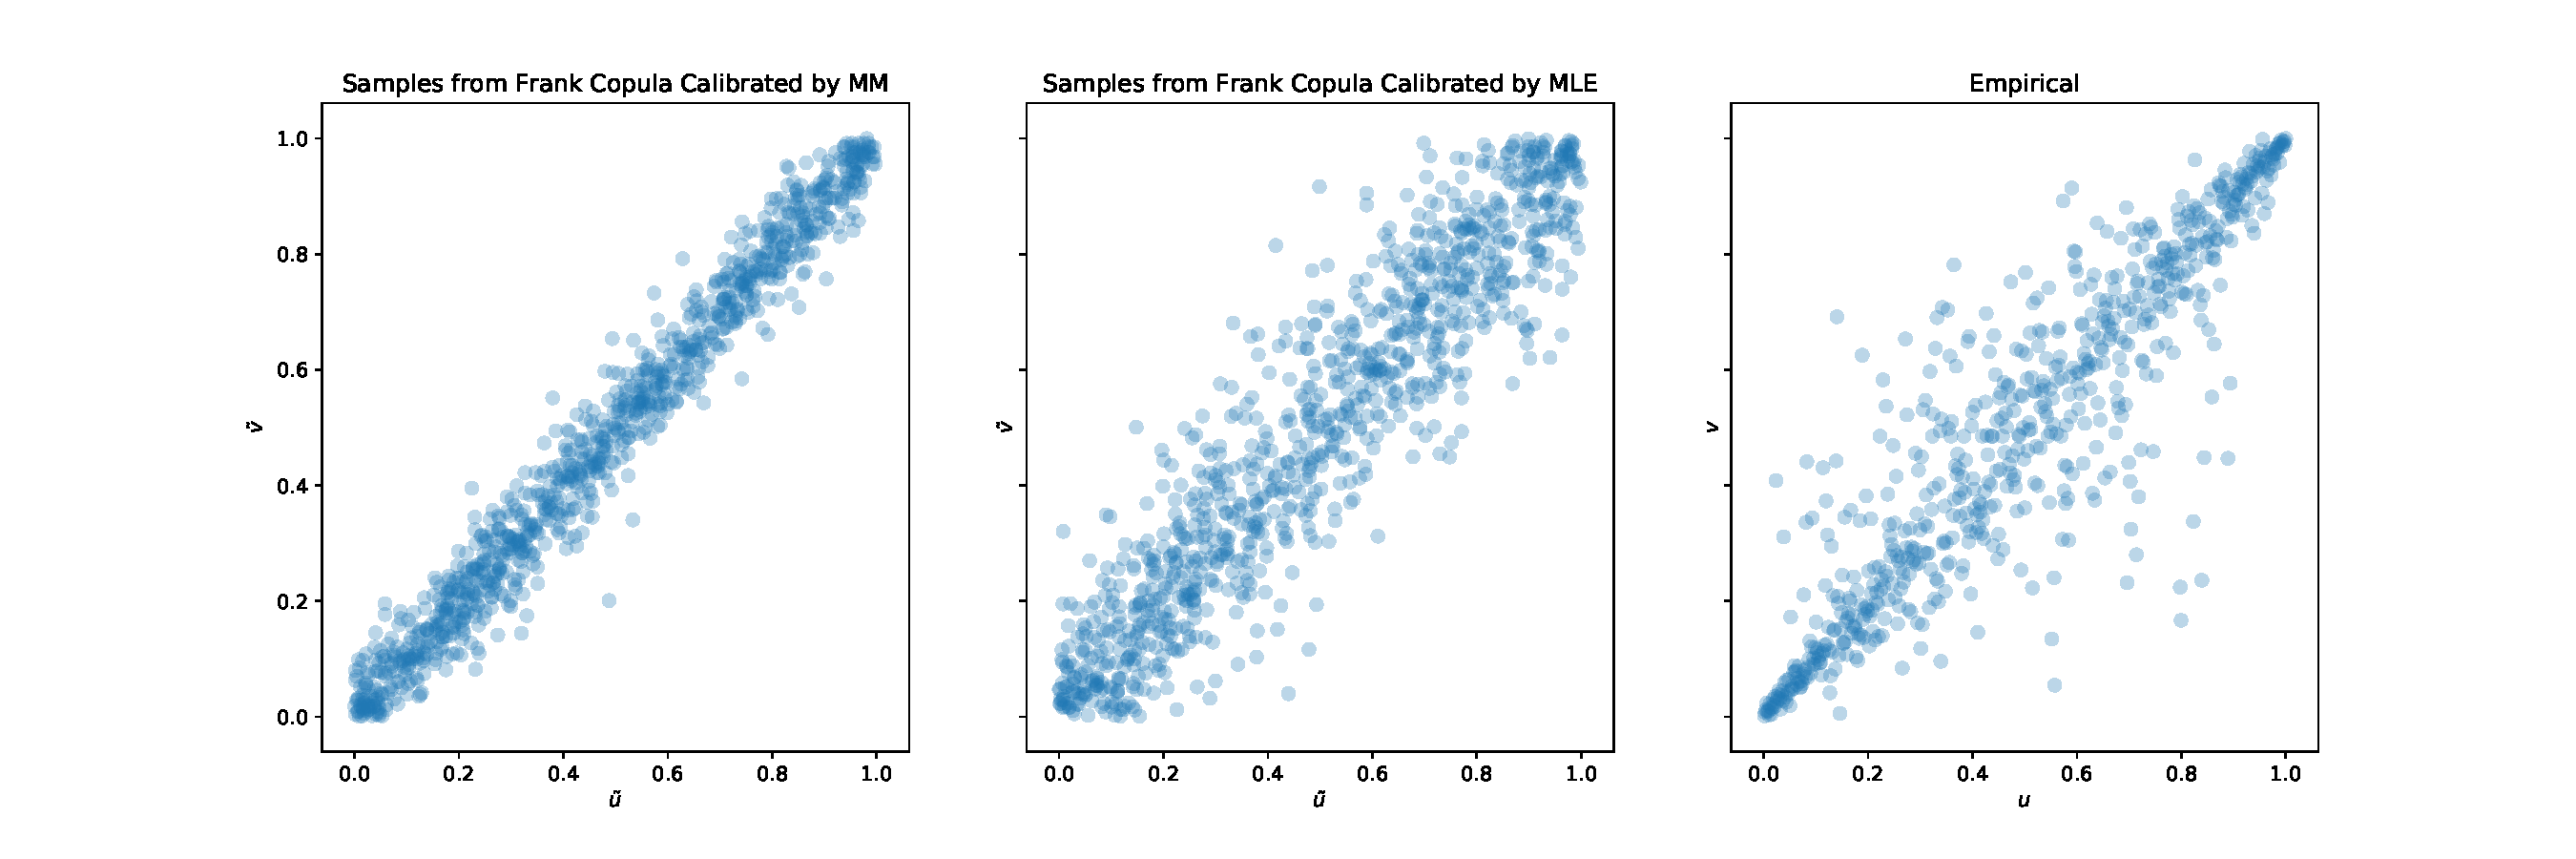
\includegraphics[width=\textwidth]{_pics/Frank.pdf}
   \caption{Comparison of Frank Copula Samples and Pseudo Observations of Bitcoin and CME Future Returns.
   \href{http://www.quantlet.com/}{
\includegraphics[width=20pt]{_pics/qletlogo_tr.png}}}
   \label{fig:Frank}
\end{figure} \medskip

Aside from the Frank-copula, the HEs of various combination of copula and risk reduction objective are very similar.
This is an expected result as the portfolio consists only two assets.
In addition to hedging effectiveness, we observe the out-of-sample returns of the hedged portfolio.
Figure~\ref{fig:OOSRH} tabulates the time series of out-of-sample returns of hedged portfolio under various copulas and risk reduction objectives. \medskip

One can see all the combinations of copula and risk reduction objective generate a large fluctuation of returns in
25/09/2019 and 26/09/2019.
This large fluctuation is due to dependence break.
\medskip

\begin{figure}[th]
   \centering
   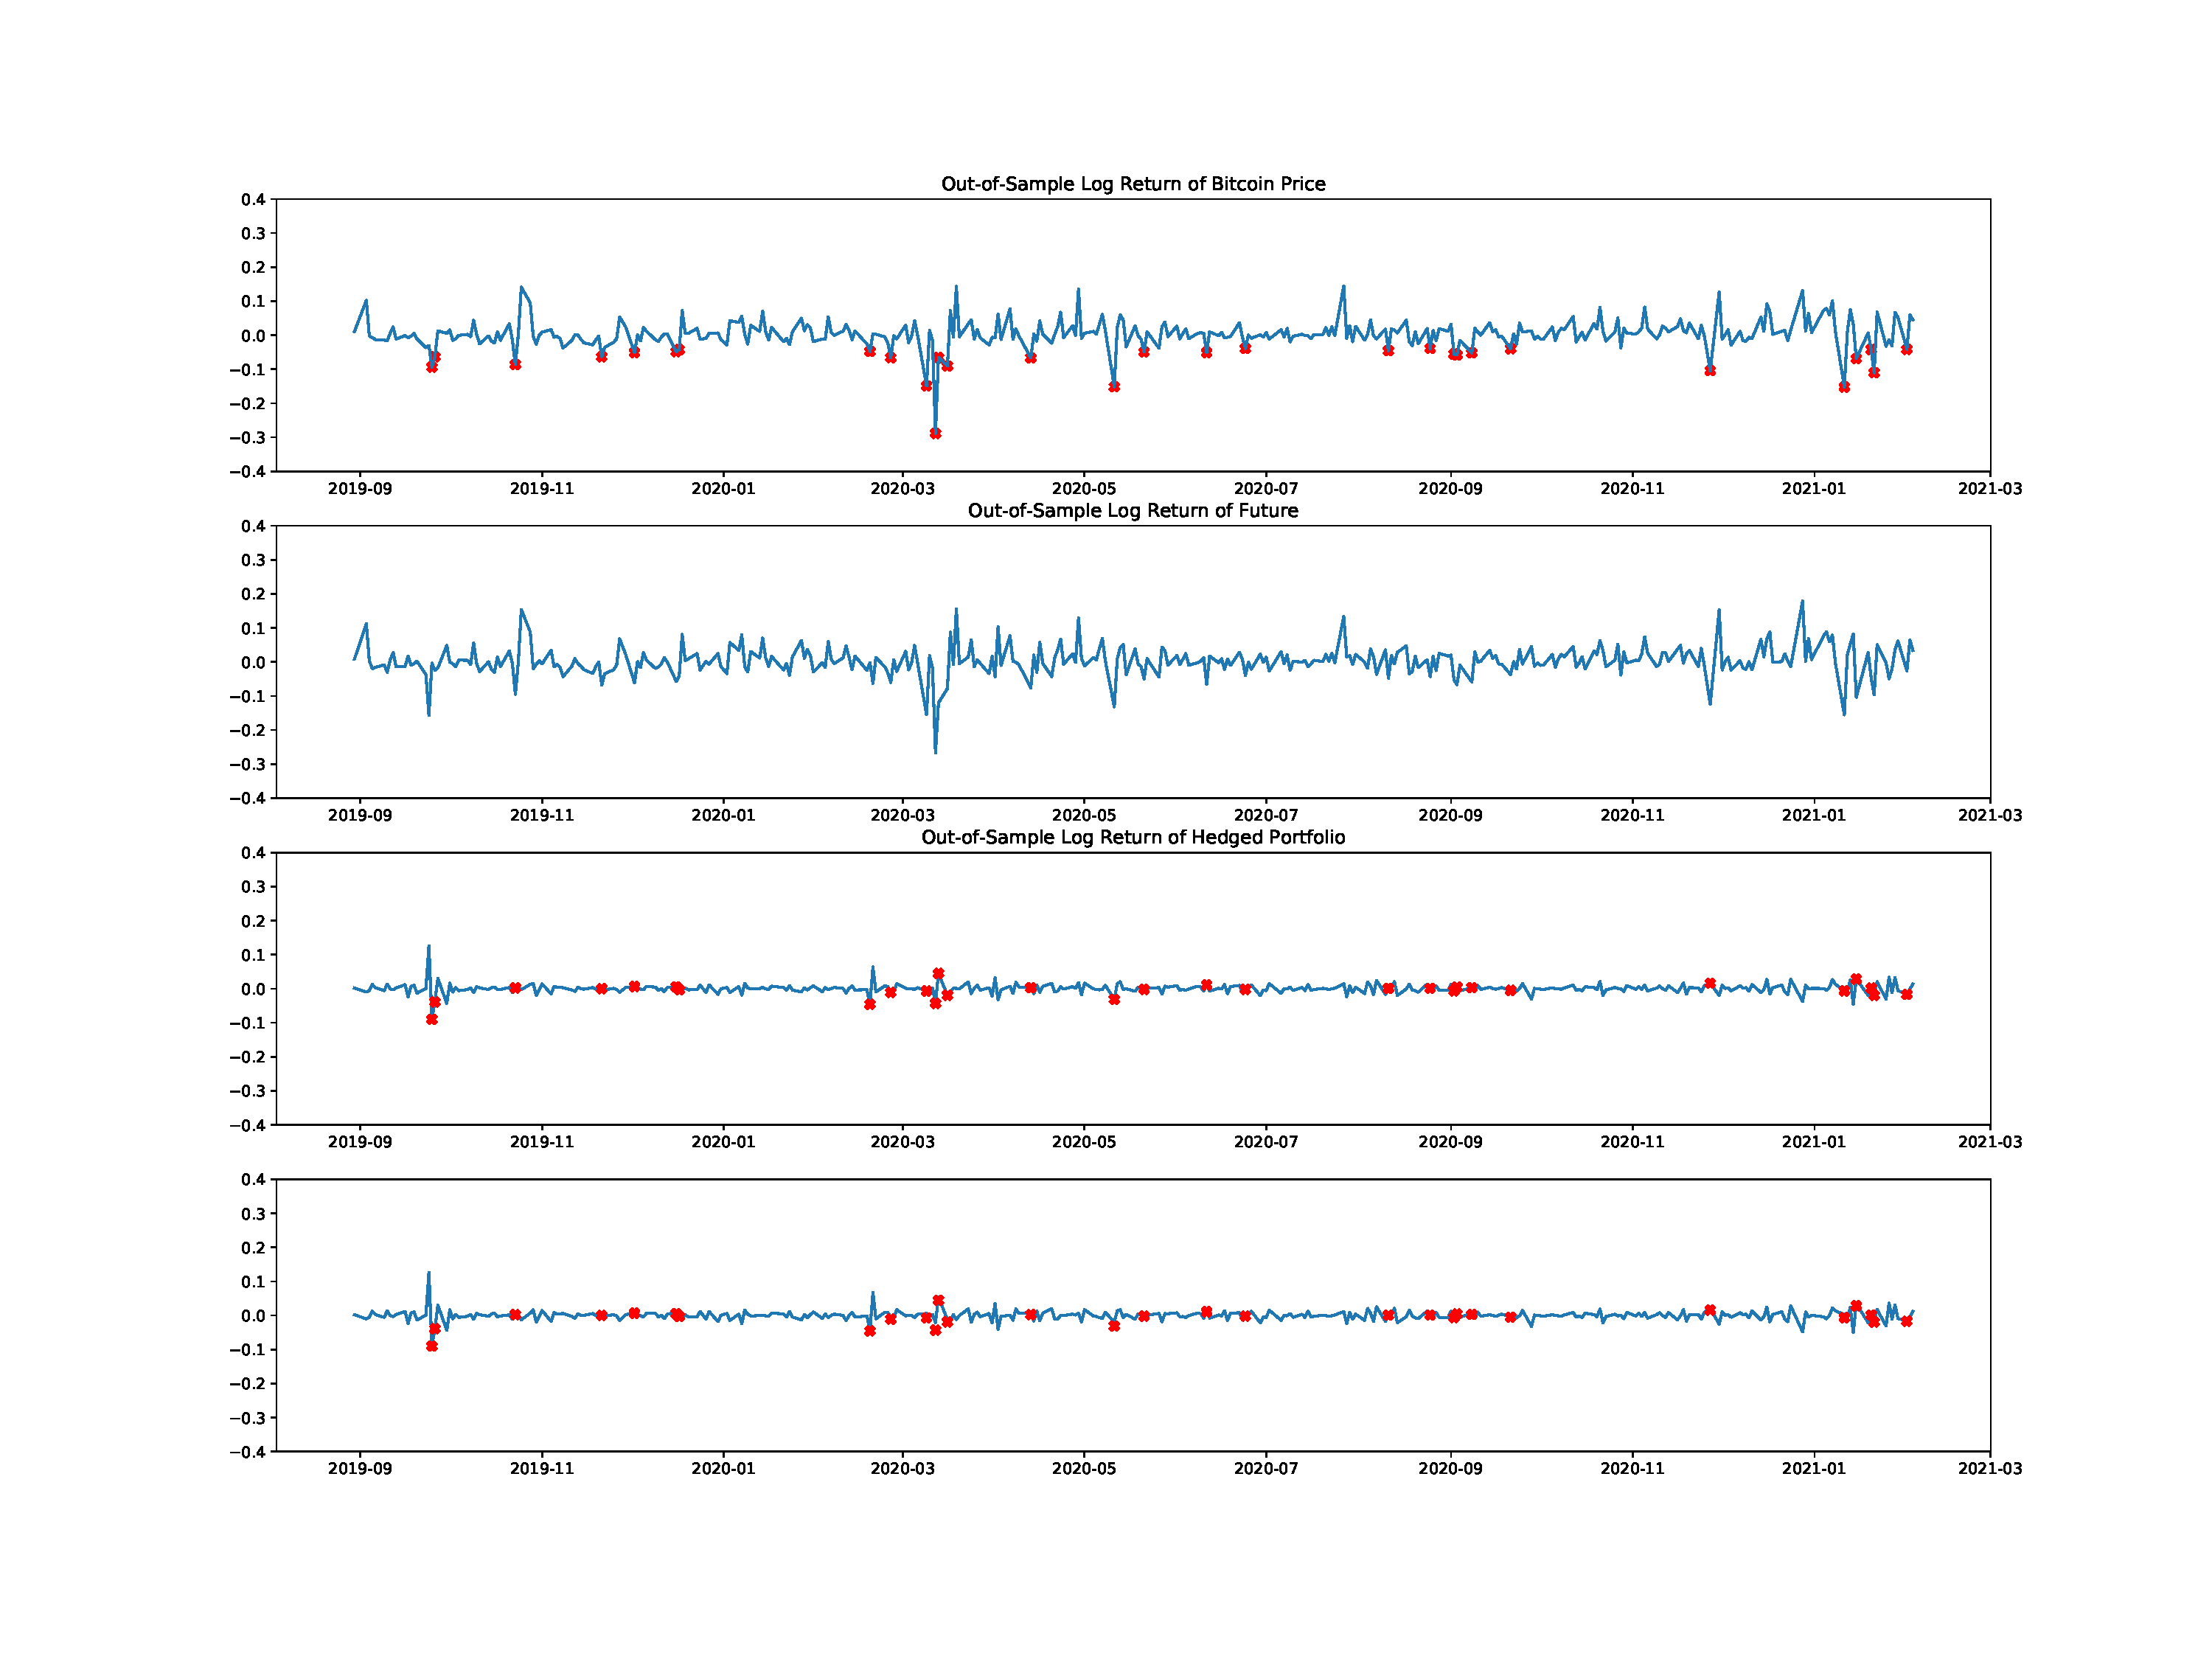
\includegraphics[width=\textwidth]{_pics/OOSreturns_compare.pdf}
   \caption{First Panel: Out of Sample Log-return of Bitcoin; Second Panel: Out of Sample Log-return of Future;
   Third Panel: Out of Sample Log-return of Hedged Portfolio by Gumbel copula with the aim of variance reduction.
   The red dots indicate the lowest 10\% return of Bitcoin, i.e. large negative moments of price.
   Forth Panel: Out of Sample Log-return of Hedged Portfolio by $h=1$ (naive hedge).
%   Lower Panel: Out of Sample Hedged Portfolio log-returns.
%   The $h^*$ is obtained from Gumbel copula aiming at reducing variance.
%   The red dots indicate the 30 most extreme negative returns in Bitcoin.
   \href{http://www.quantlet.com/}{
\includegraphics[width=20pt]{_pics/qletlogo_tr.png}}}
   \label{fig:Gumbel}
\end{figure}

\newpage
\begin{landscape}
\begin{figure}[th]
   \centering
   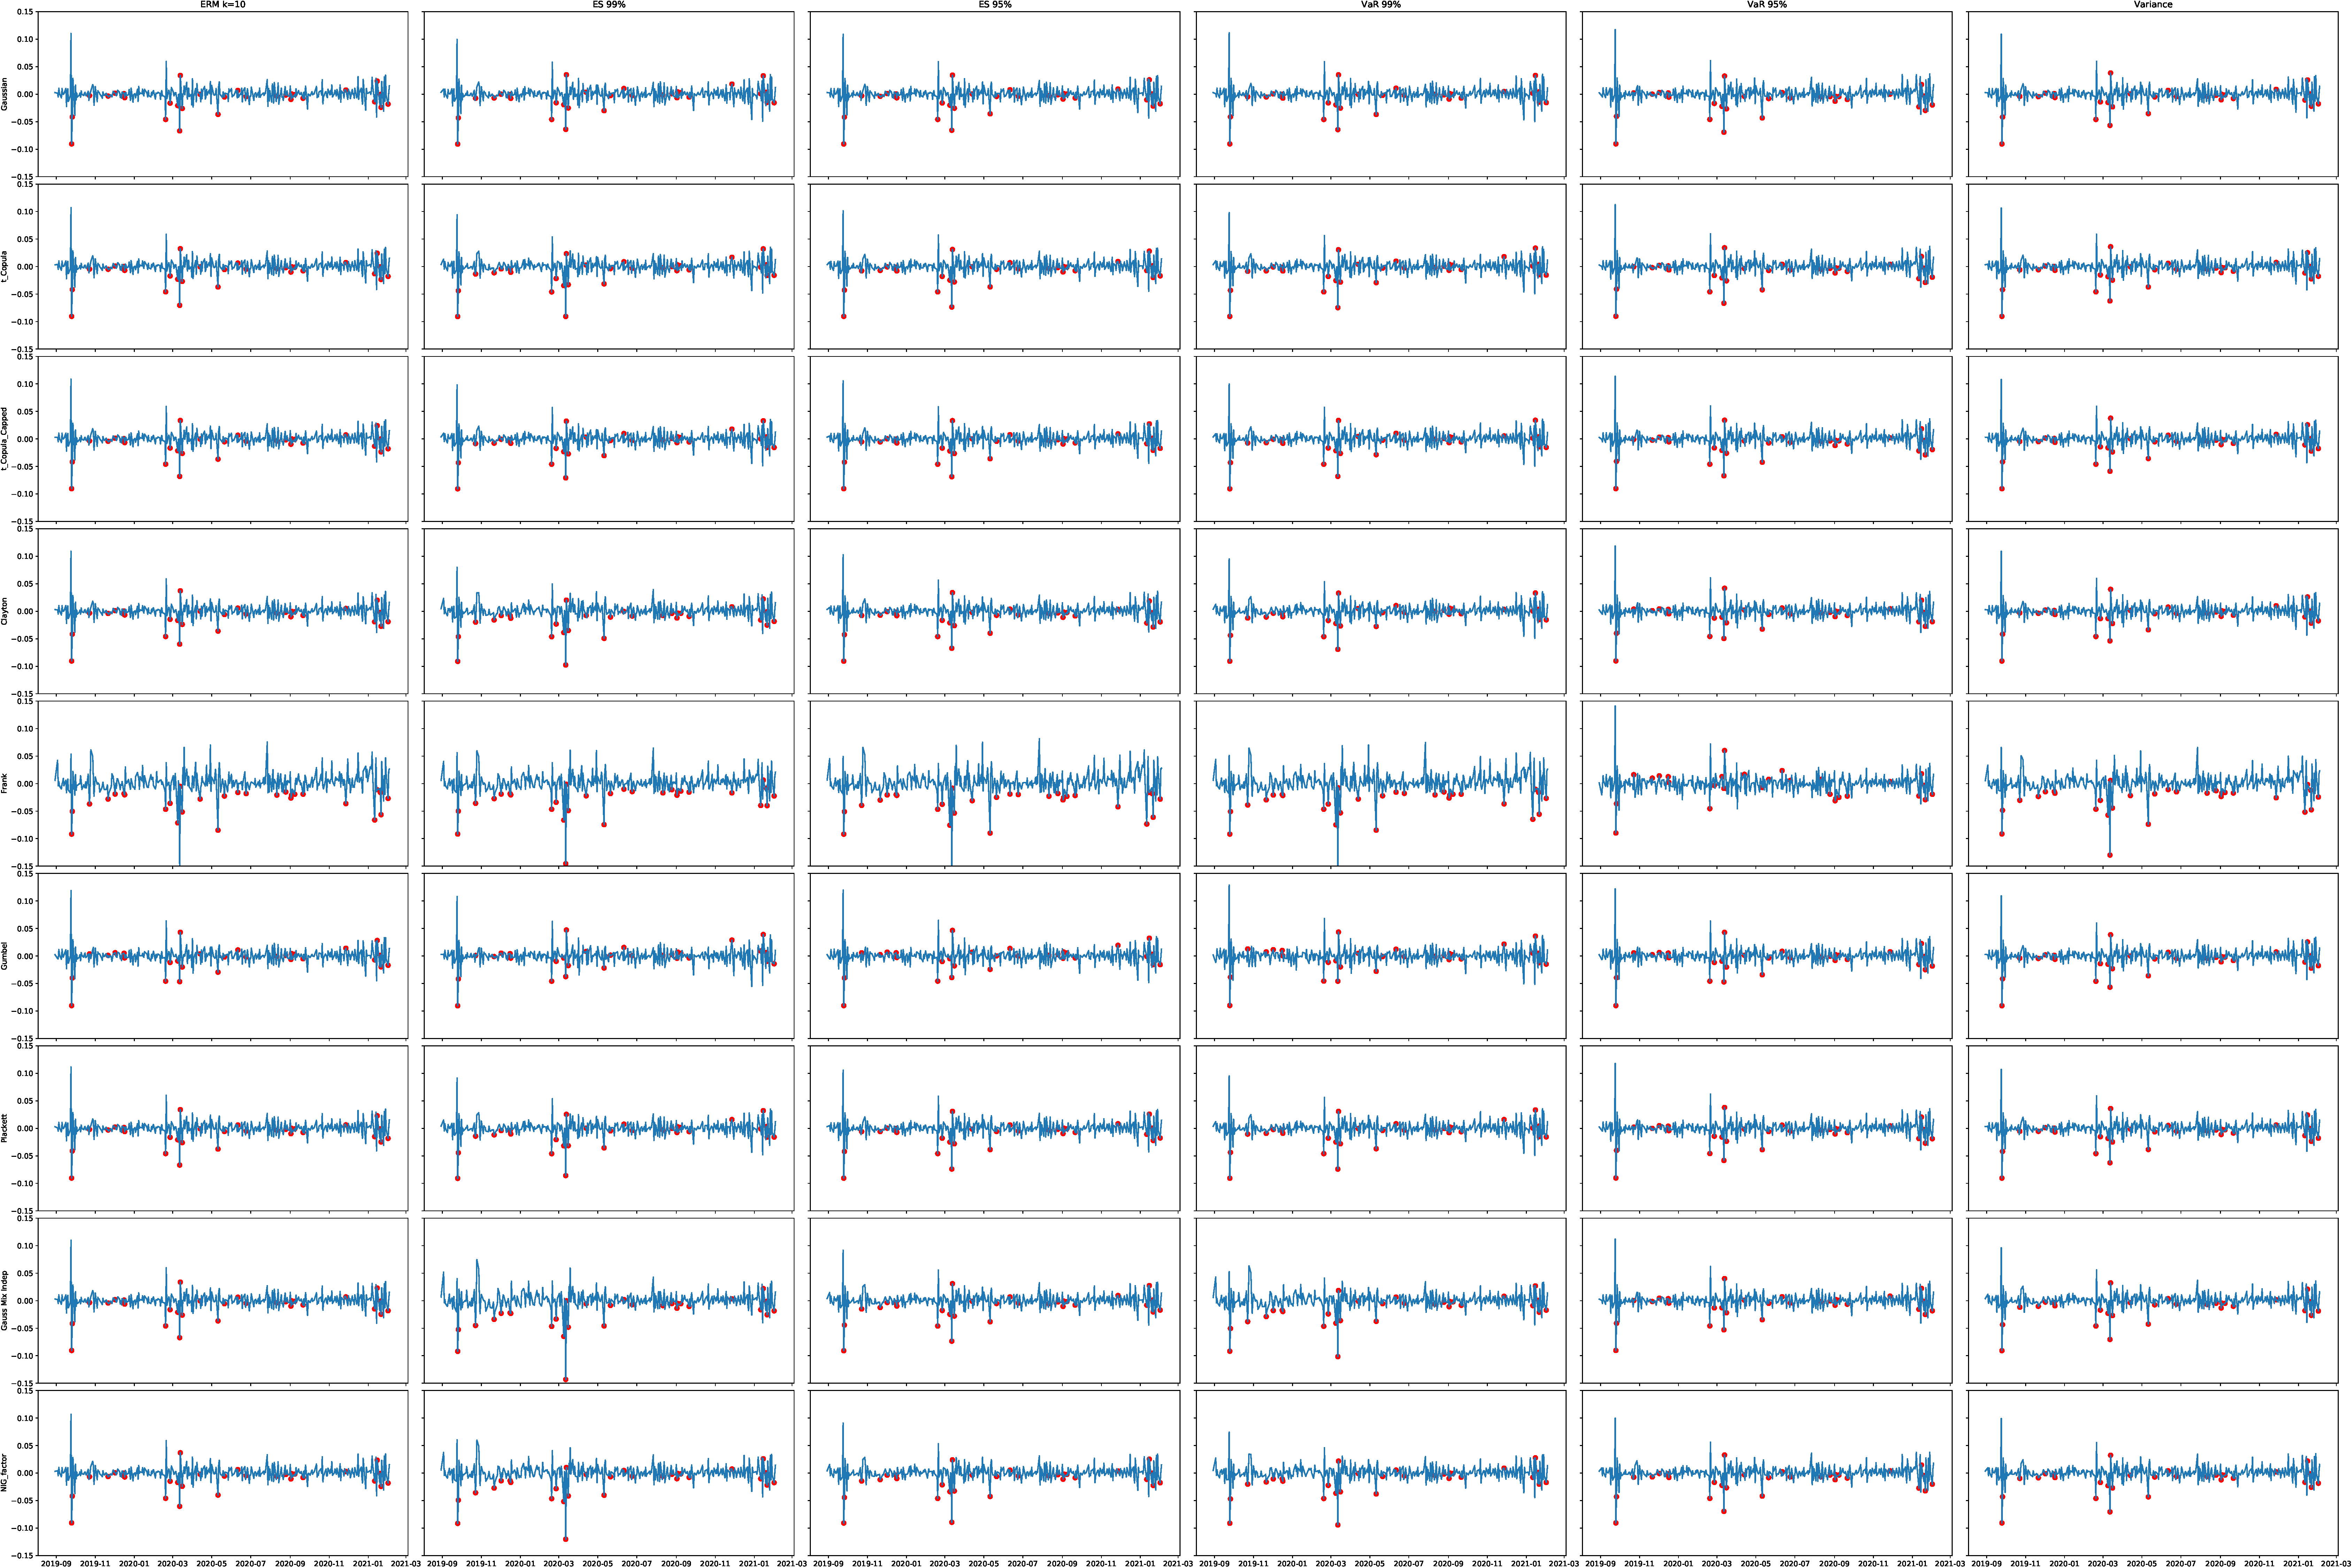
\includegraphics[width=\linewidth]{_pics/Rhs.pdf}
   \caption{Out-of-Sample Returns of Hedged Portfolio of Copulas and Risk Reduction Objectives.
   \href{http://www.quantlet.com/}{
\includegraphics[width=20pt]{_pics/qletlogo_tr.png}}}
   \label{fig:OOSRH}
\end{figure}
\end{landscape}
\newpage

\newpage
\begin{landscape}
\begin{figure}[th]
   \centering
   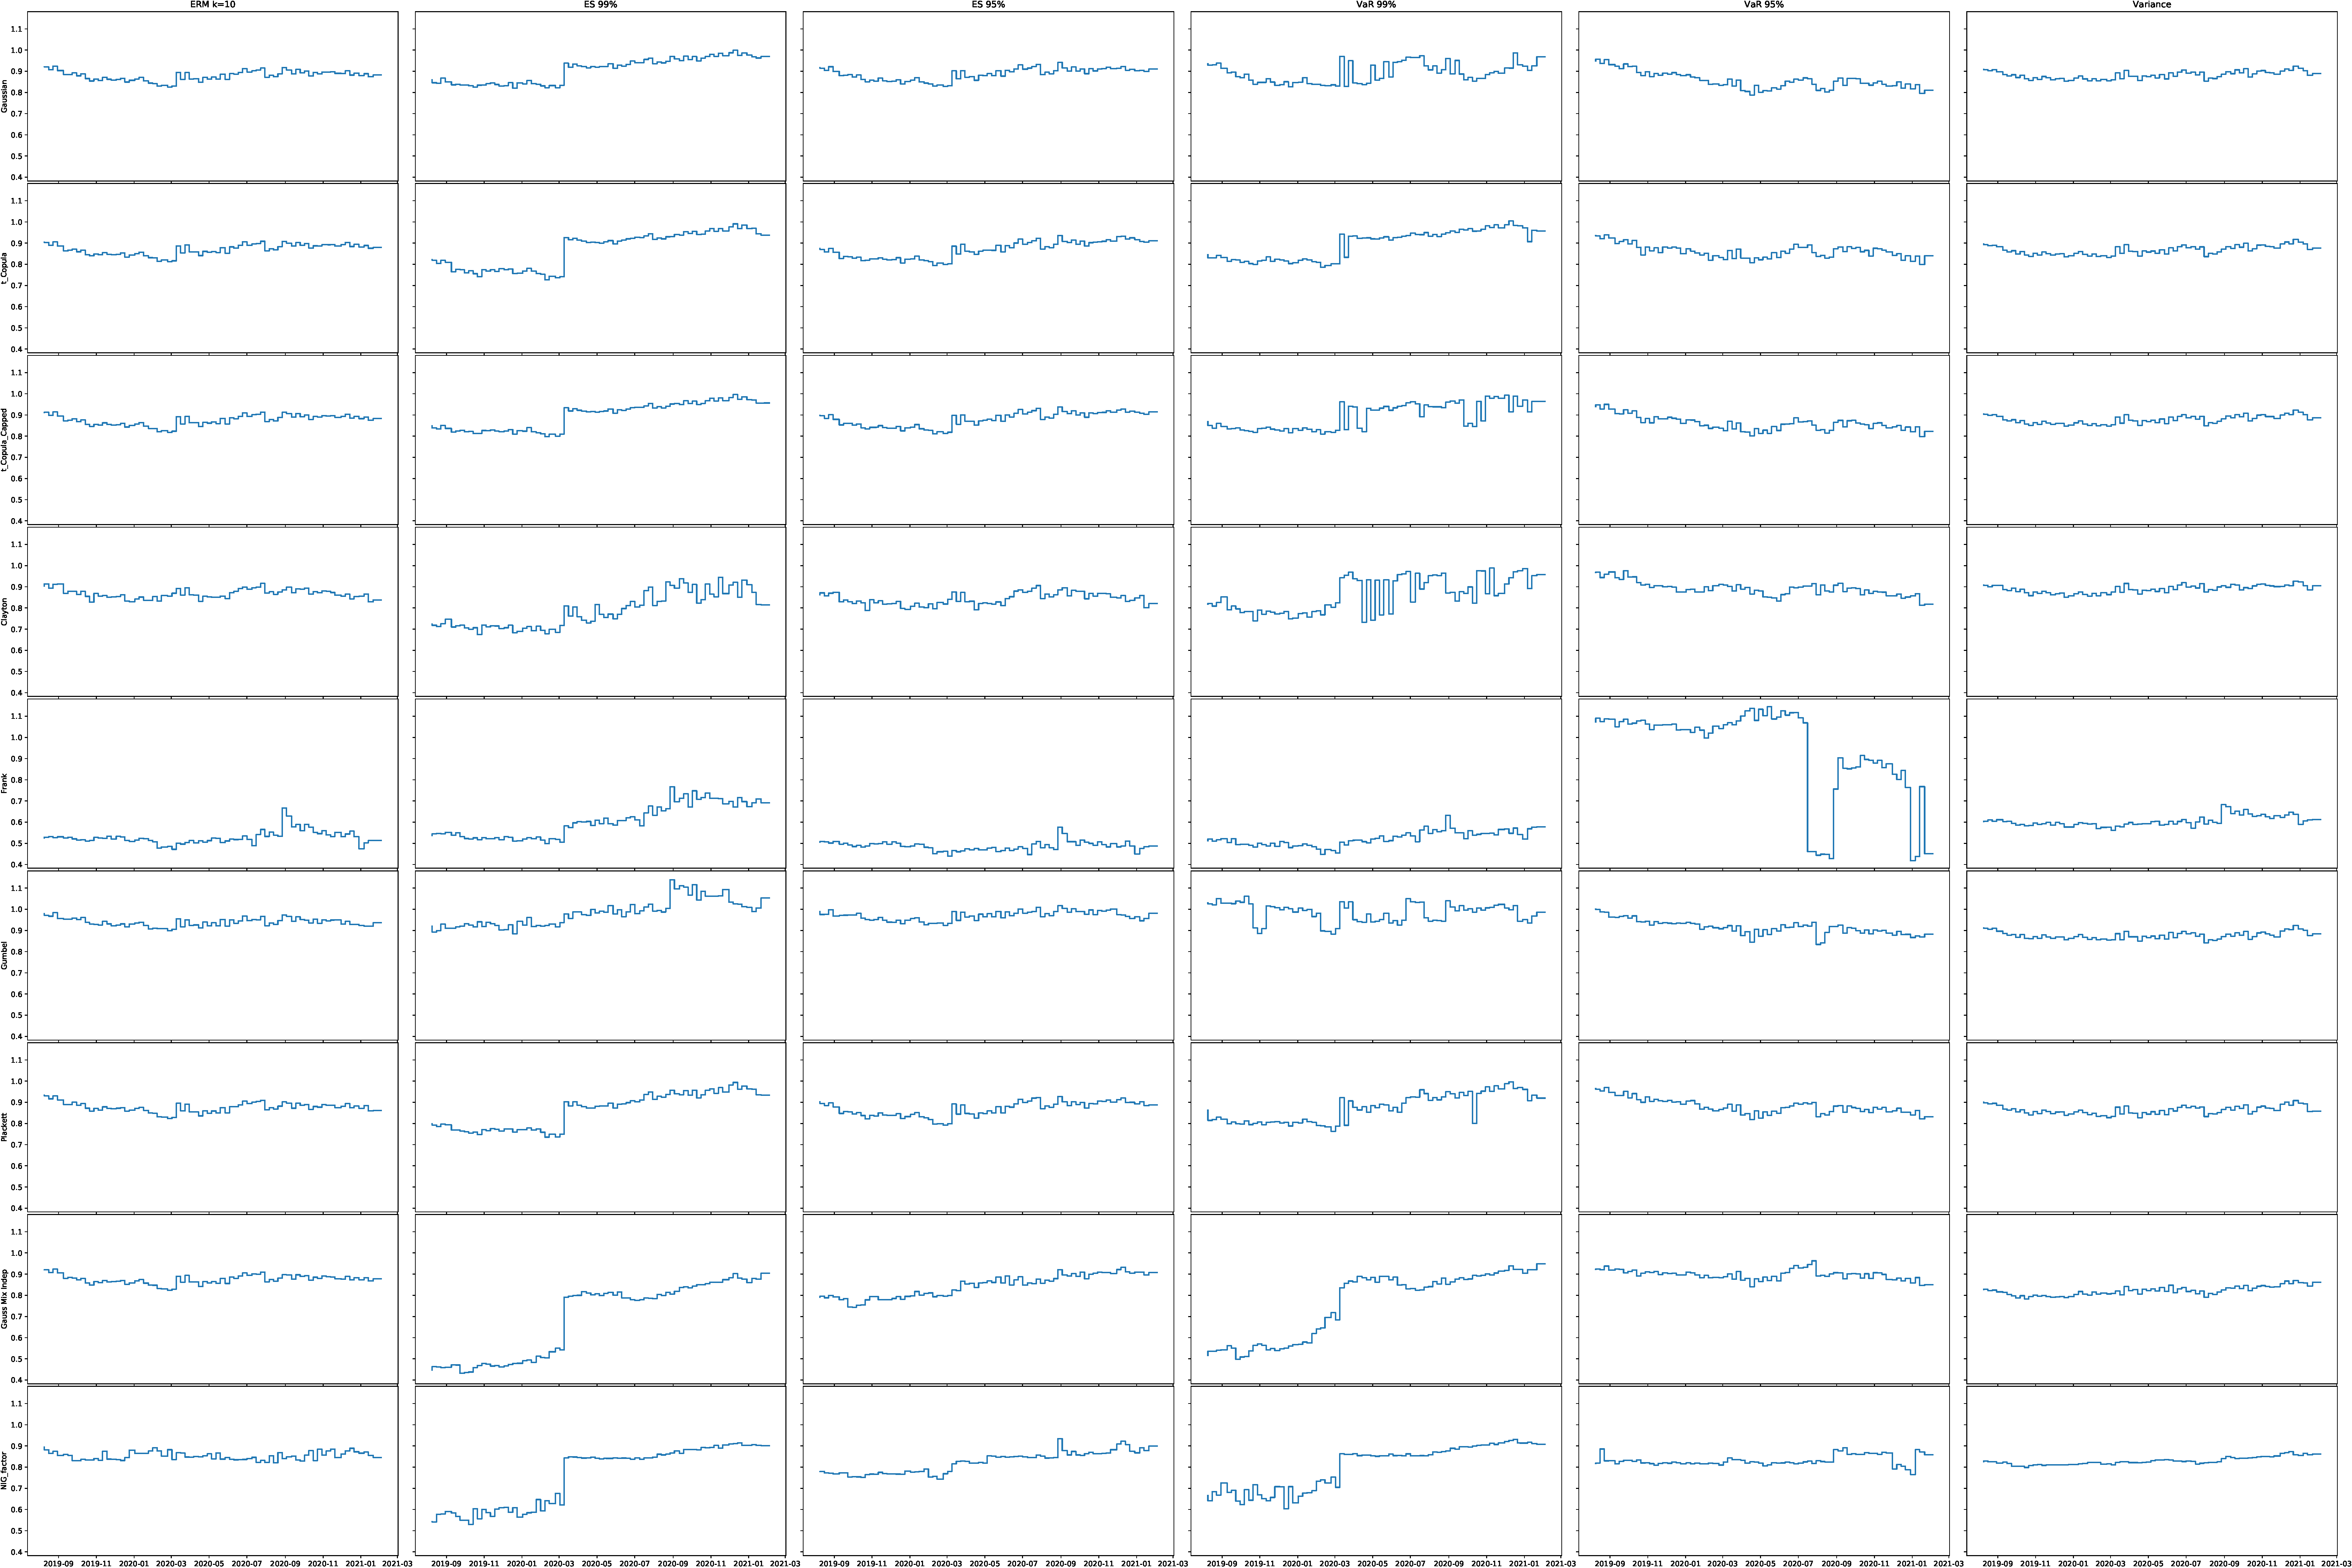
\includegraphics[width=\linewidth]{_pics/OHRs.pdf}
   \caption{Optimal Hedge Ratio Obtained from Combinations of Copula and Risk Reduction Objective.
   \href{http://www.quantlet.com/}{
\includegraphics[width=20pt]{_pics/qletlogo_tr.png}}}
   \label{fig:OHRs}
\end{figure}
\end{landscape}
\newpage


%\begin{figure}[t]
%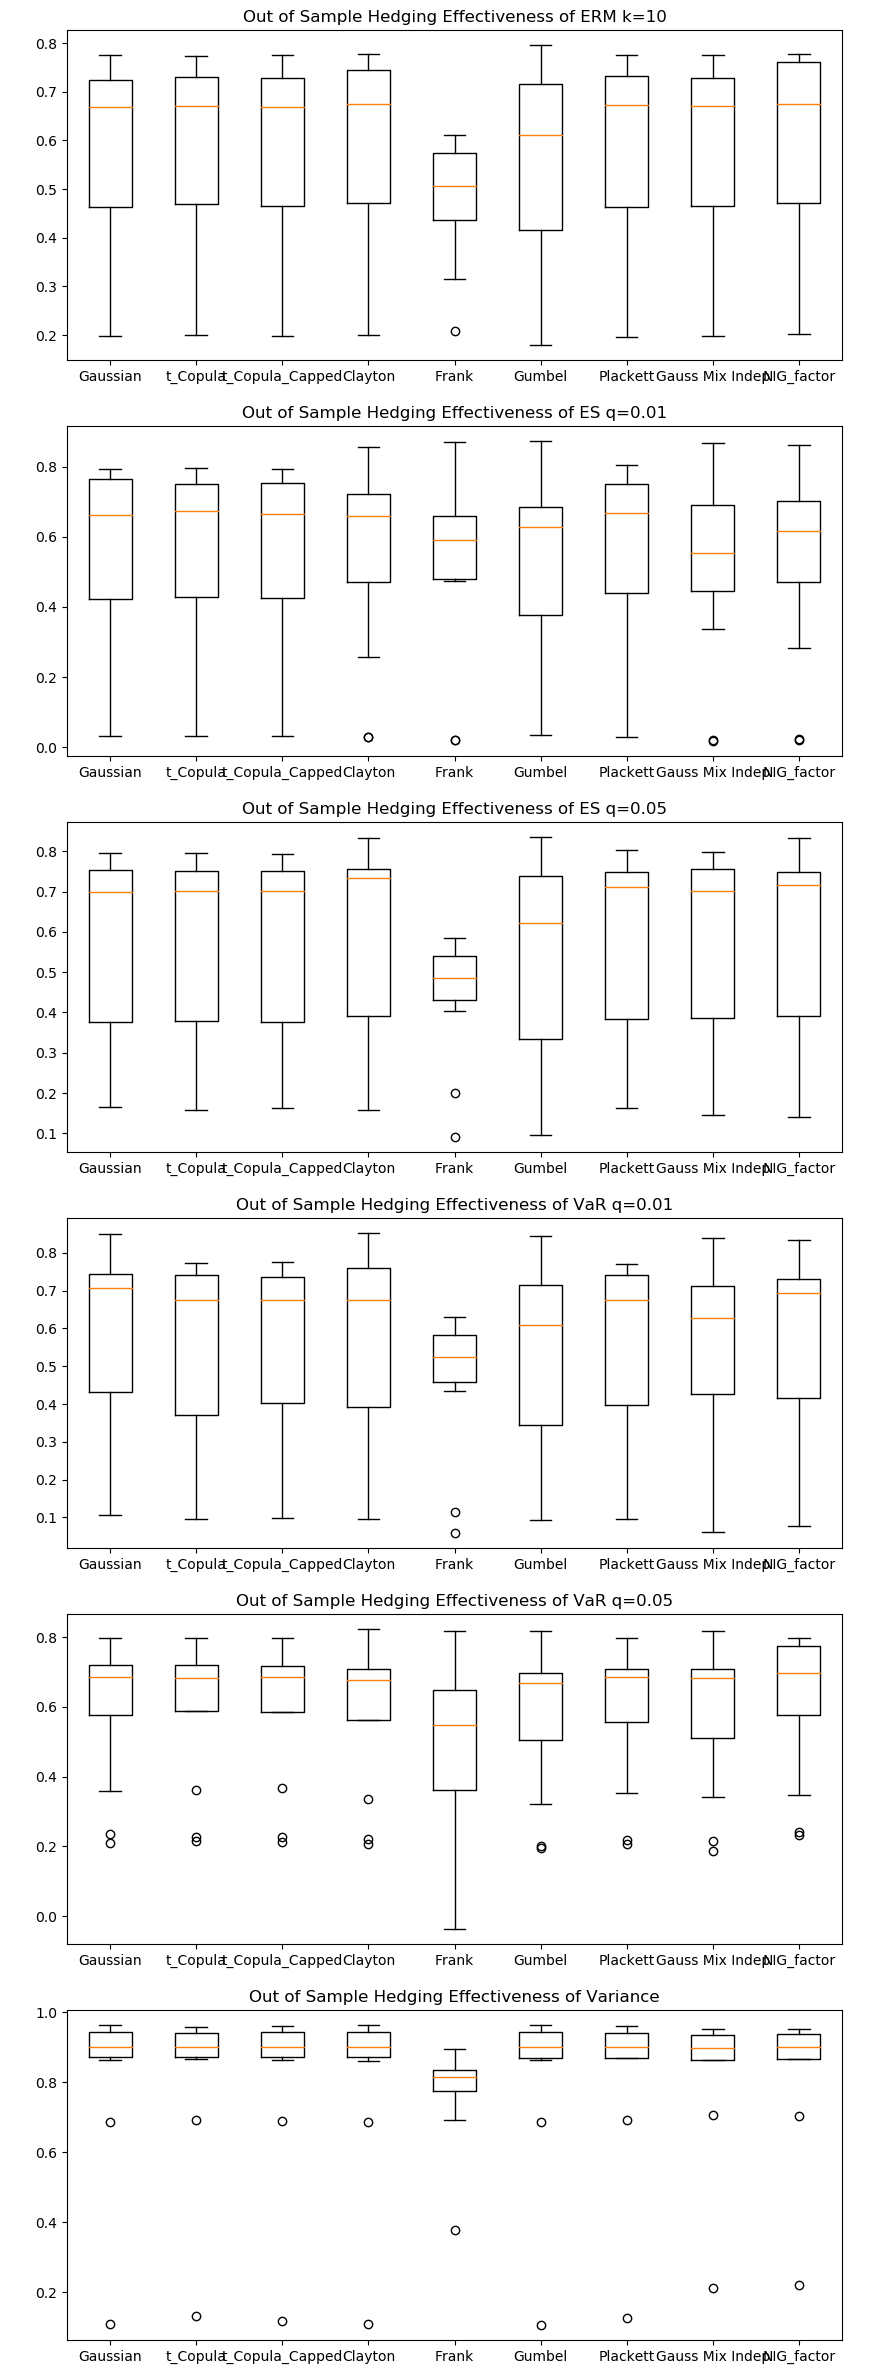
\includegraphics[width=\textwidth, height=\textheight]{_pics/Out of Sample Hedging Effectiveness.png}
%  \caption{}
%\label{out of Sample Hedging Effectieness}
%\end{figure}

\begin{figure}[H]
   \centering
   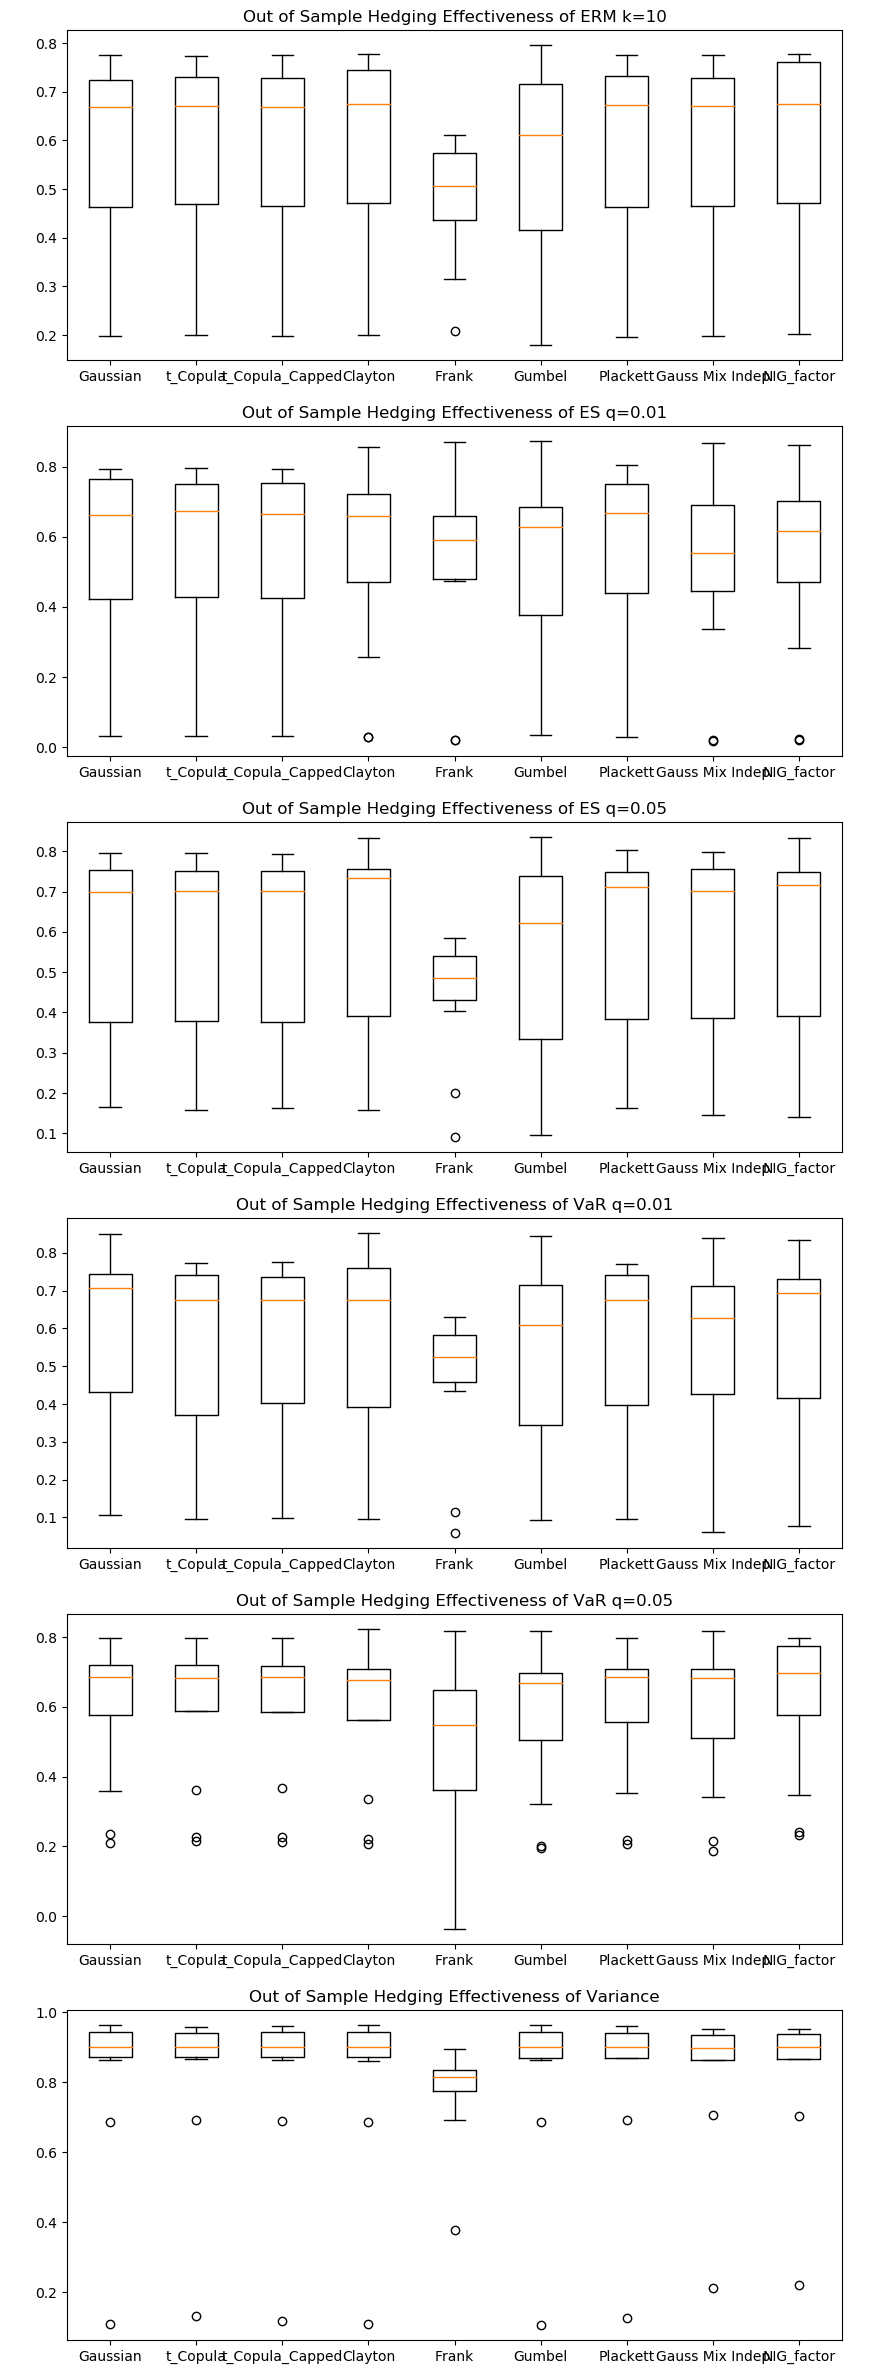
\includegraphics[height=24cm]{_pics/Out of Sample Hedging Effectiveness.png}
   \caption{Out of Sample Hedging Effectiveness Box-plot.
   The HEs are obtained from a set of out-of-sample data,
   each set consists 30 days log returns of Bitcoin and CME future.
   \href{http://www.quantlet.com/}{
\includegraphics[width=20pt]{_pics/qletlogo_tr.png}}}
   \label{fig:OOSHE}
\end{figure}

Figure~\ref{fig:Gumbel} shows the time series of out-of-sample $r^h$ using Gumbel copula with the
objective of reducing variance.
The red dots are the 30 most extreme negative returns in Bitcoin.
In the figure, we can see the downside risk of Bitcoin is well managed by the hedging procedure with Gumbel copula.
Most of the extreme losses of Bitcoin are greatly reduced by introducing the CME future in the hedged portfolio.
Two exceptions are found in 25/09/2019 and 26/09/2019, where the CME future failed to follow the large drop in Bitcoin. (TODO: drop reason)
One of the possible reason is that traders was performing rollover activities on 25-26/09/2019, which
27/09/2019 is the expiry day of the September future.
Another reason for Gumbel fail of capturing the loss is dependence break.
The Kendall's tau in the training data is 0.2 higher than that of the testing data.
Other copulas suffer from the break as well.



%\subsection{Stability of $h^*$}
\subsection{Robustness}\label{subsec:robustness}
The study of robustness concerns the stability of statistical estimation procedure under the existence of outliers.
This has an economical meaning to our hedging exercise: Do we want the optimal hedge ratio react to extreme market changes?
In practice, outliers of returns can come from anywhere, for example, a tweet from Elon Musk, a sudden large order from
institutional investor, or an incident of system failure in cryptocurrency exchanges.
Rapid and drastic changes in portfolio weight causes problem of slippage and transaction cost.
Investors should be aware of the cost brought by the sensitivity of the optimal hedge ratio procedure.
\medskip

The discussion of sensitivity or robustness dates back to \citet{huber1981robust}'s work on robust statistics.
\citet{hampel2011robust} suggest an infinitesimal approach to investigate sensitivity of statistical procedures.
There are three central concepts in this approach, qualitative robustness, influence function, and break-down point.
They are loosely related to the concept of continuity, first derivative of functional, and the distance of a functional to its nearest pole (singularity).
While the first concept is a qualitative feature of a functional, the second the third concepts are practical tools to measure sensitivity quantitatively.
We deploy a finite sample version of the second and third concepts.
Details of robustness of risk measures can be found in \citet{cont2010robustness}. \medskip

\francis{\em [FL: Need to rewrite the following to show the IF of hedge performance instead of h. But Please have a look of the methodology first.]}
With a probability space $(\Omega, \F, \p)$,
we denote $M: \Omega \mapsto \mathscr{C}, M \in \{\text{MLE}, \text{MM}, \text{Empirical}\}$ be estimators of interest for distribution of returns,
$\mathscr{C} = \{\text{Gaussian-Copula}, ..., \text{Plackett-Copula}, \text{Empirical-Copula}\} \in \p$ be a set of bivariate distributions of interest,
$\rho_{h}: \mathscr{C} \mapsto \mathbb{R}$ be a risk measure on the hedged portfolio given $h$,
and finally, $\hat h_\rho = \argmin_h \rho_{h} \circ M$ be a functional to obtain the optimal hedge ratio (OHR) depending on risk measure
$\rho$. \medskip

The influence function of $\hat h_\rho$ with finite sample size $n$ is
\begin{align}
    \text{IF}(\bm{z}; \hat h_\rho) = \frac{\hat h_\rho(\bm{X}_1,...,\bm{X}_n, \bm{z})-
    \hat h_\rho(\bm{X}_1,...,\bm{X}_n)}{\frac{1}{n+1}}.
    \end{align}

\francis{\em [The inclusion of $\bm{z}$ has nothing to do with the probability in a probability space, i.e. it is possible to include points with density zero.]}

The equation describes the effect of a single contamination at point $\bm{z}$ on the estimate of OHR,
standardised by the mass of the contamination. \medskip

Figure~\ref{fig:IFs} shows the influence function of $\hat h_\rho$ of using $t$ copula estimated by MLE with 300 data points of
Bitcoin and CME future returns from 14/12/2018 to 25/02/2020.
Contamination are $[-0.3,-0.27,..., 0.3] \bigotimes [-0.3,-0.27,..., 0.3]$, in total $900$ pairs of contamination. \medskip

We can see from the plots that Expected Shortfall with $\alpha = 99\%$ is very sensitive the negative return in spot (lower right plot).
The $h^*$ obtained this way increases with a single contamination of negative jump in spot price.
VaR at $99\%$ is also sensitive to negative jump in spot price but with a lower level (lower left plot).
This is a natural result that reflect investor's risk strong preference of avoidance: investor increase her future's short position
to compensate potential large drop in spot price.
The result of ES being more sensitive to VaR as risk measure agrees with the conclusion of \citet{cont2010robustness}. \medskip

Other risk measures are relatively less sensitive.
Interestingly, although ERM place heavy weights to negative returns,
its IF is similar to that of variance, where variance does not exhibit risk preference.
\francis{[FL:This might due to the smooth $\phi(p)$ over the spectrum $[0,1]$ of ERM. The $\phi(p)$ of VaR is a Dirac function at a single point $\alpha$, that of ES
has a sharp cut off at $1-\alpha$, a tiny change in rank of $r^h$ causes VaR and ES to shift their weights.]}


\begin{figure}[h!t]
      \centering
   \begin{tabular}[width=20cm, height=20cm]{ccc}
             \centering
   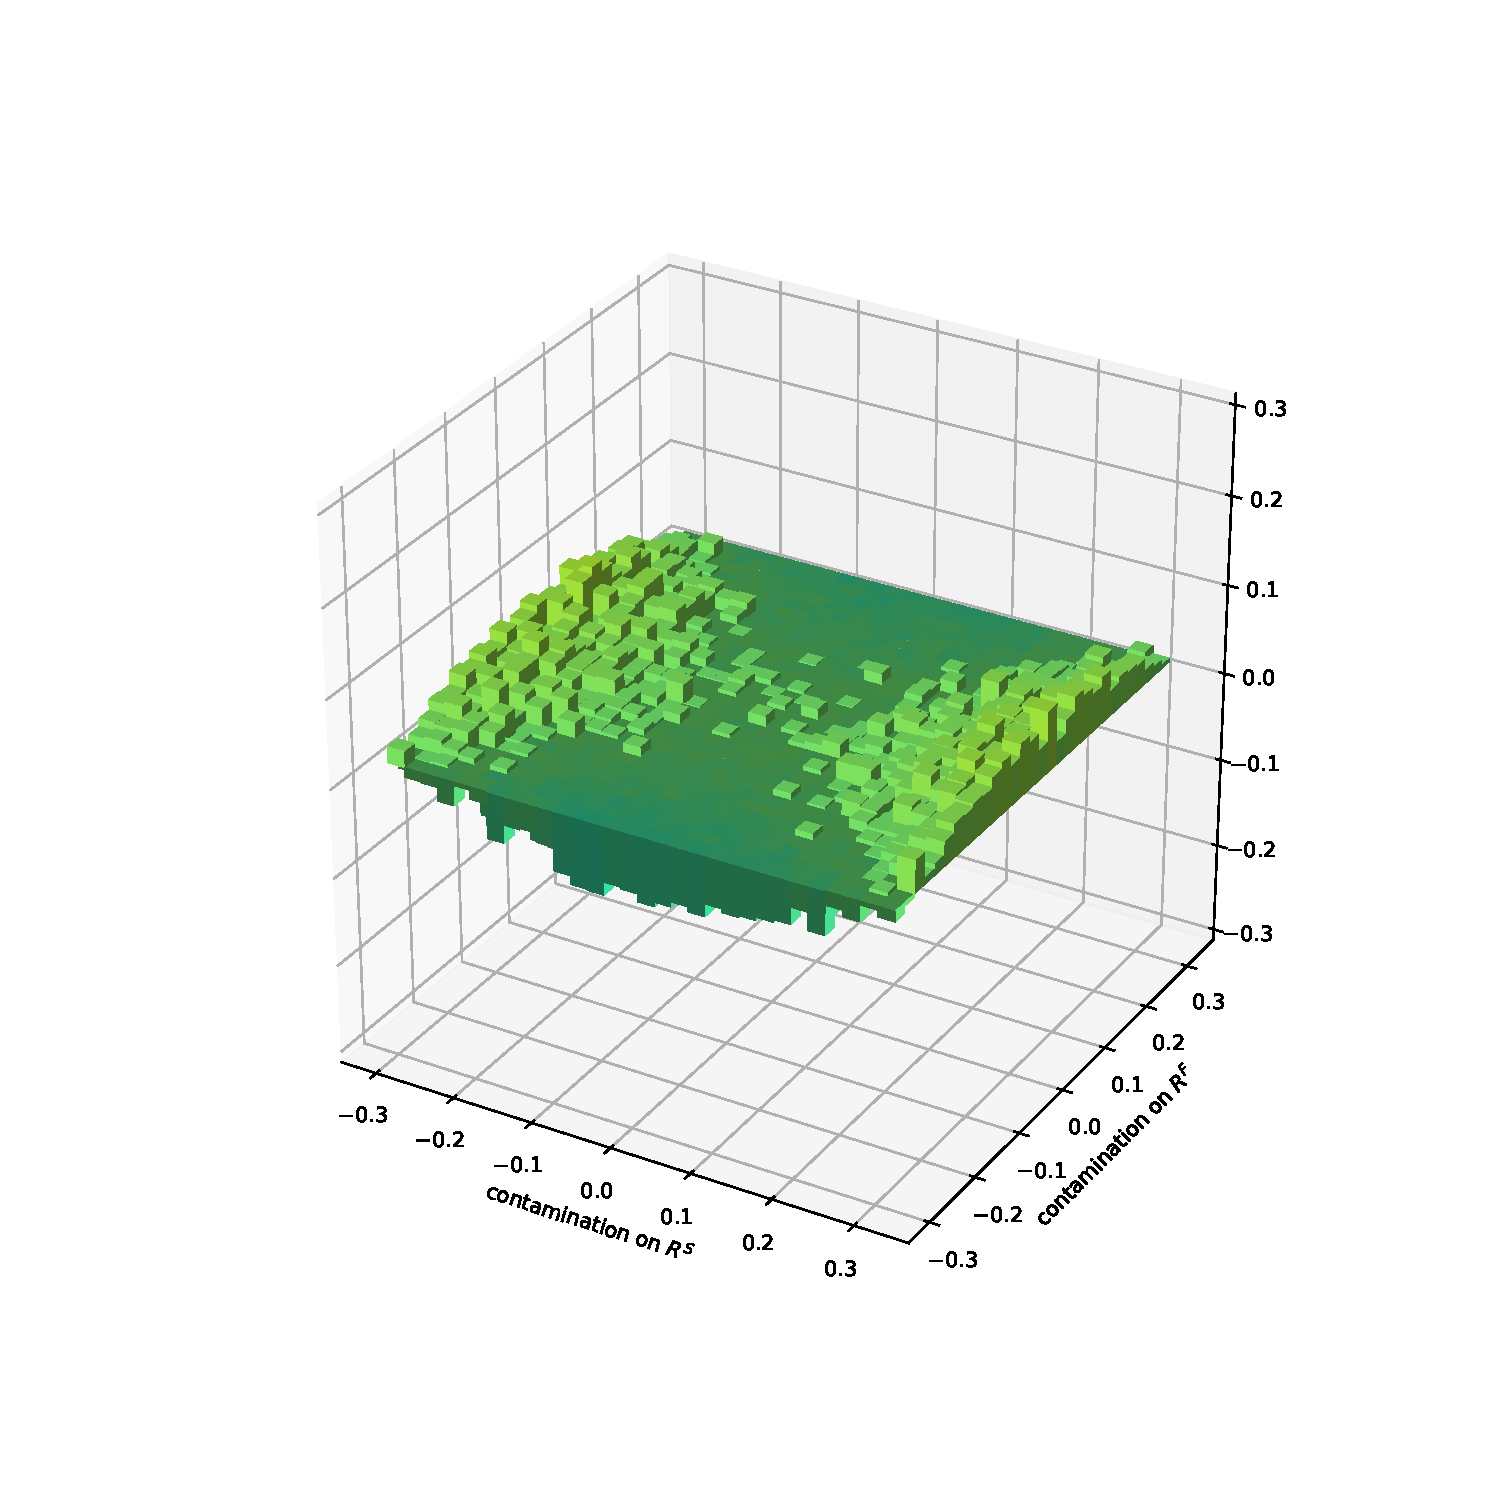
\includegraphics[height=5cm]{_pics/IF_plots/Variance_t_copula_MLE.pdf} &
   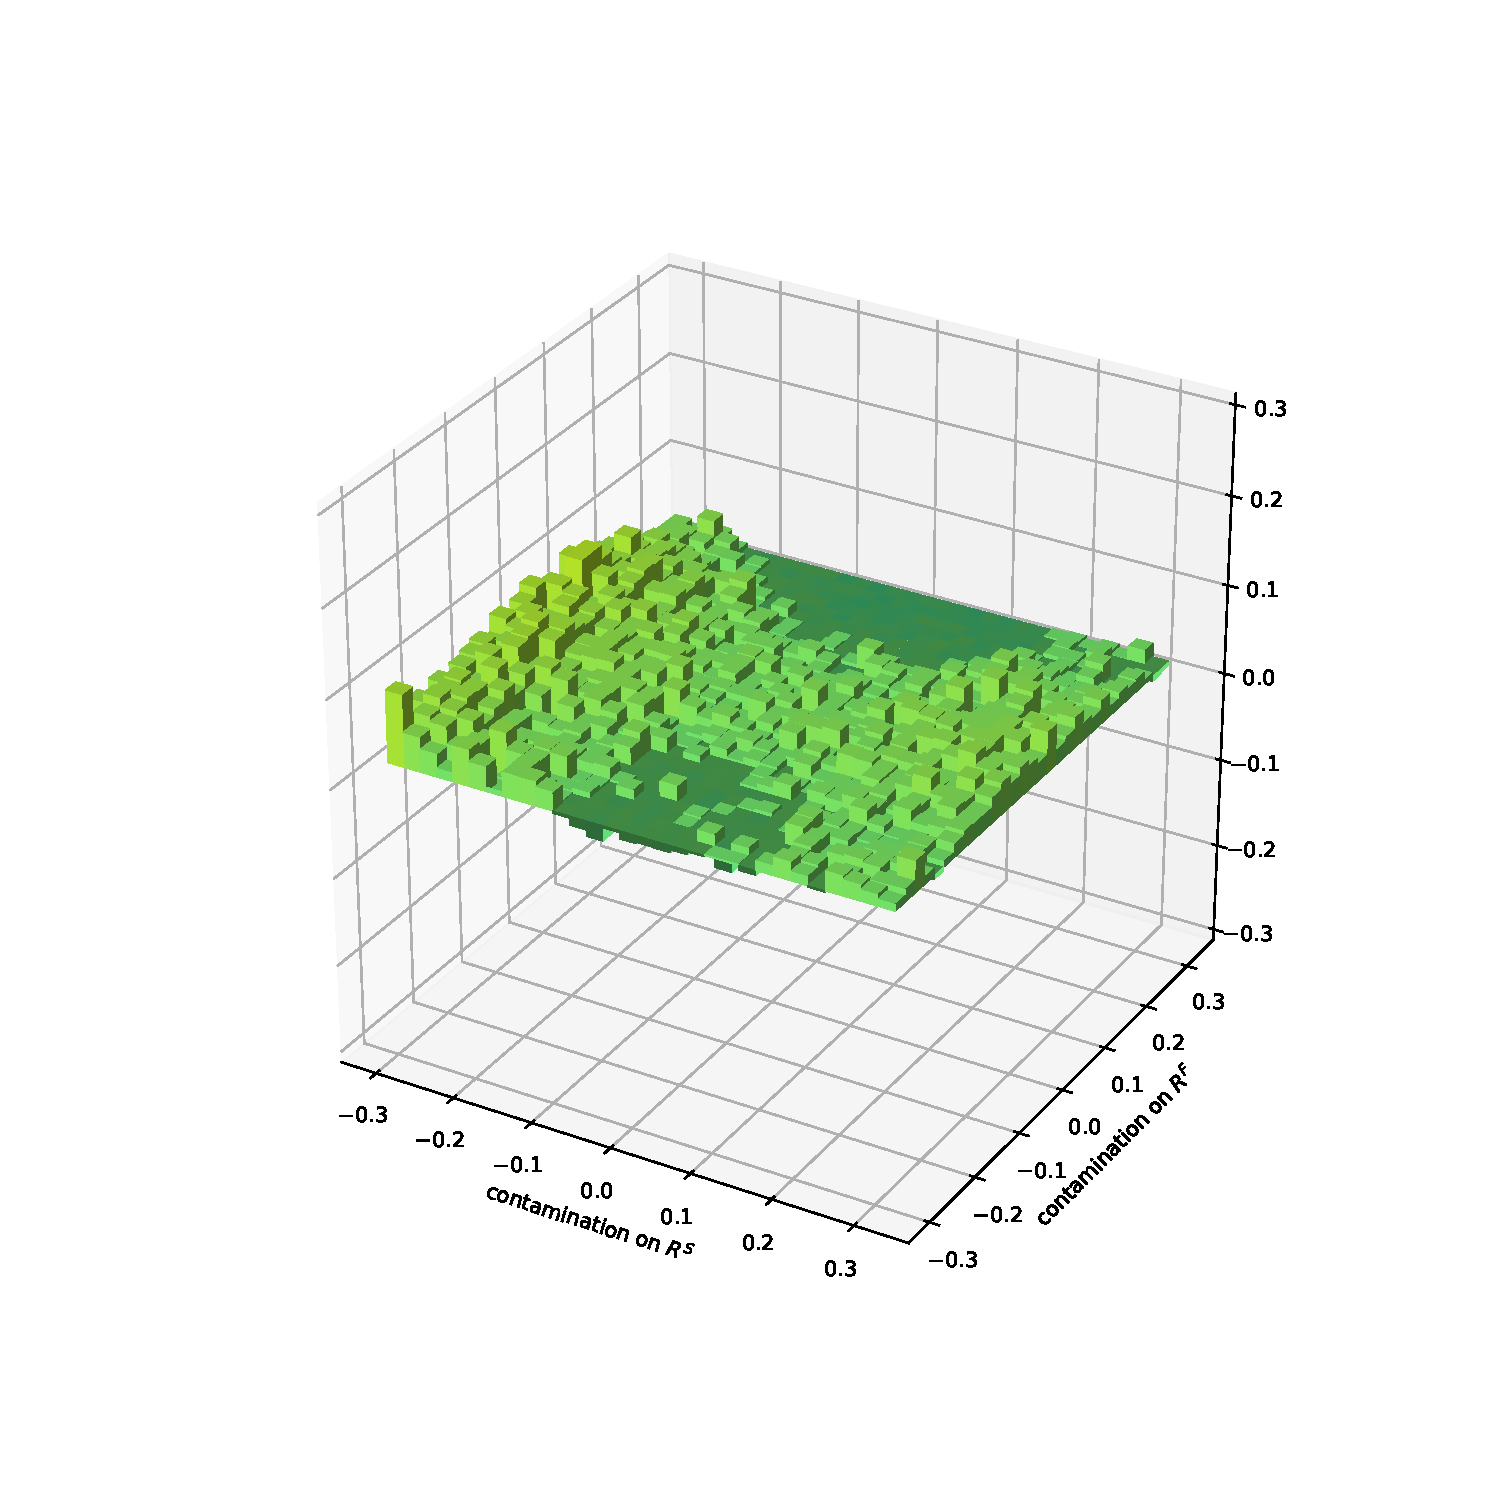
\includegraphics[height=5cm]{_pics/IF_plots/ERM10_t_copula_MLE.pdf}&
   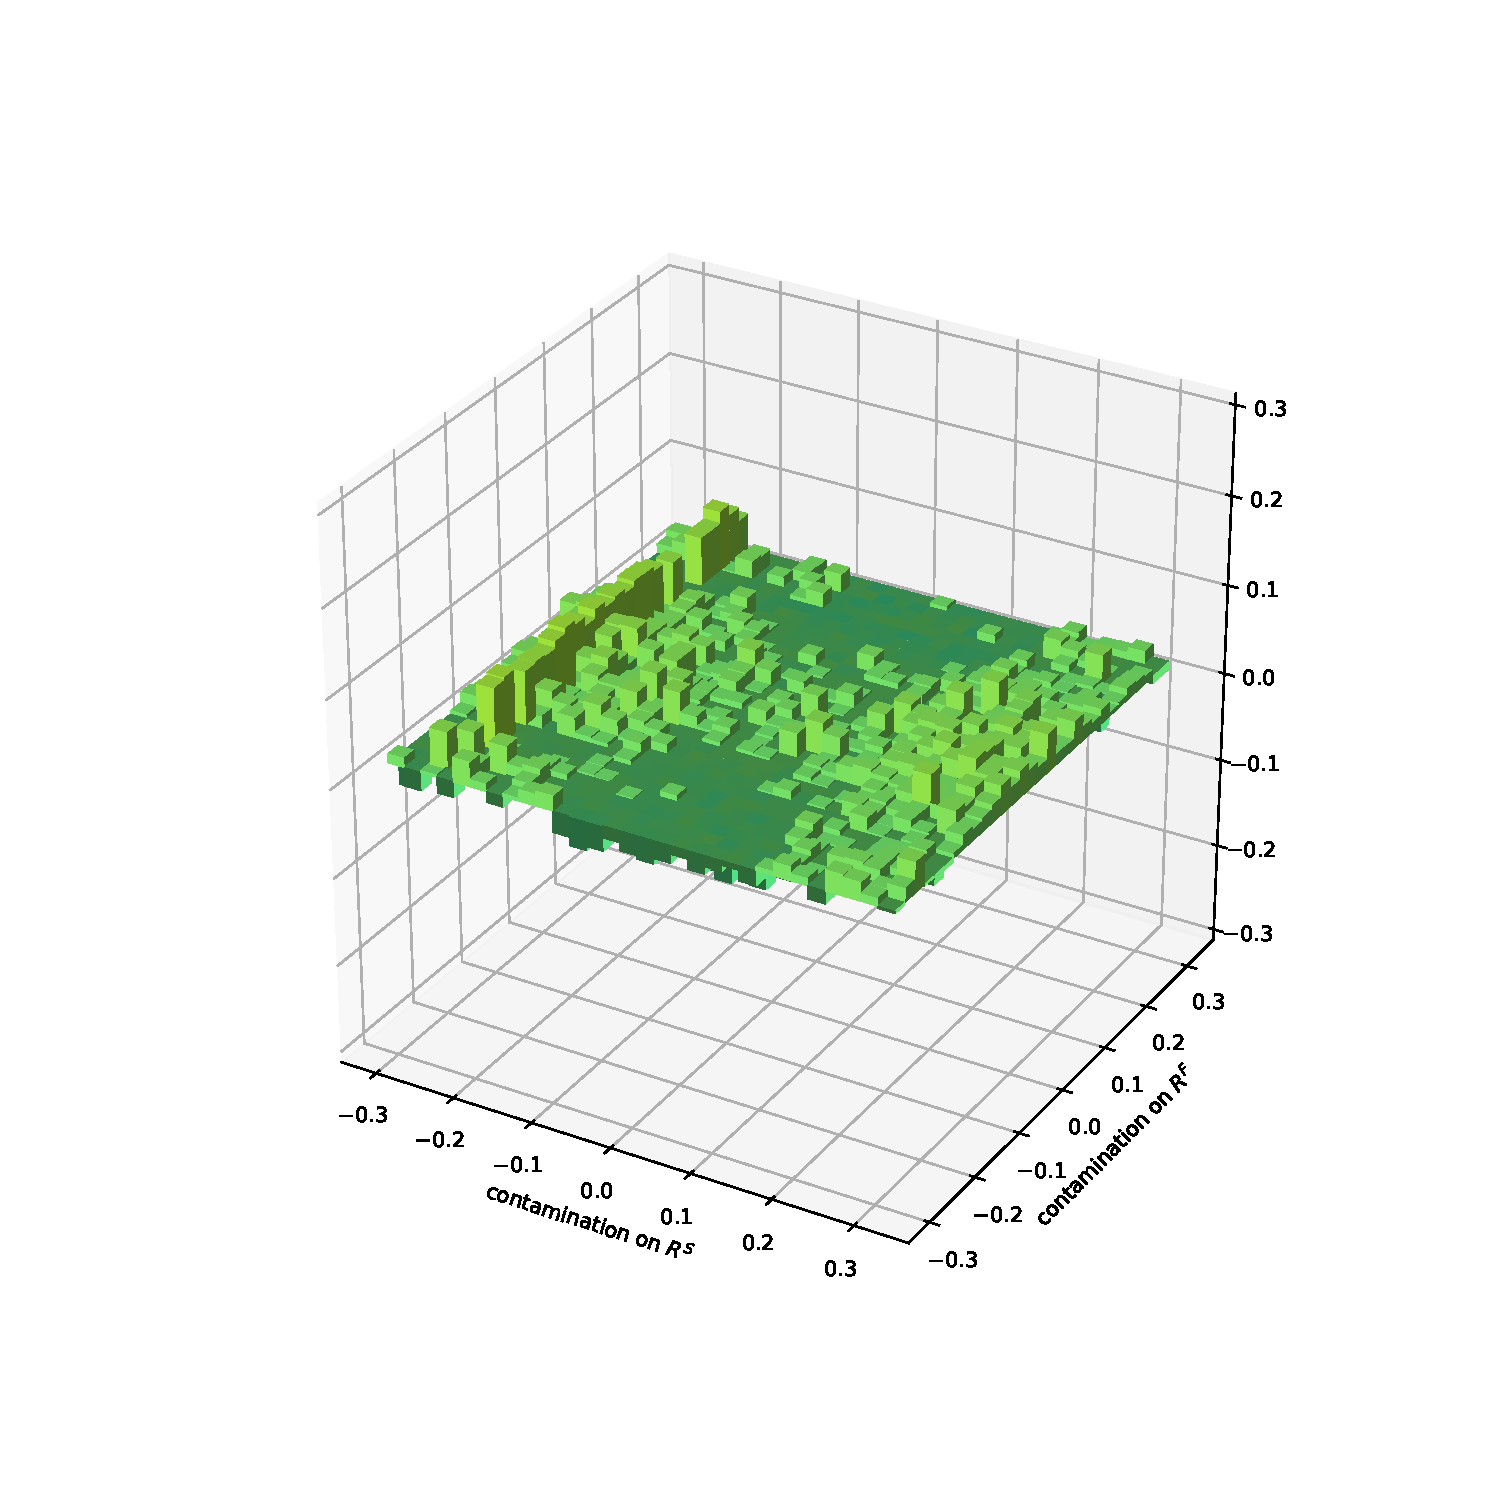
\includegraphics[height=5cm]{_pics/IF_plots/VaR5_t_copula_MLE.pdf} \\
   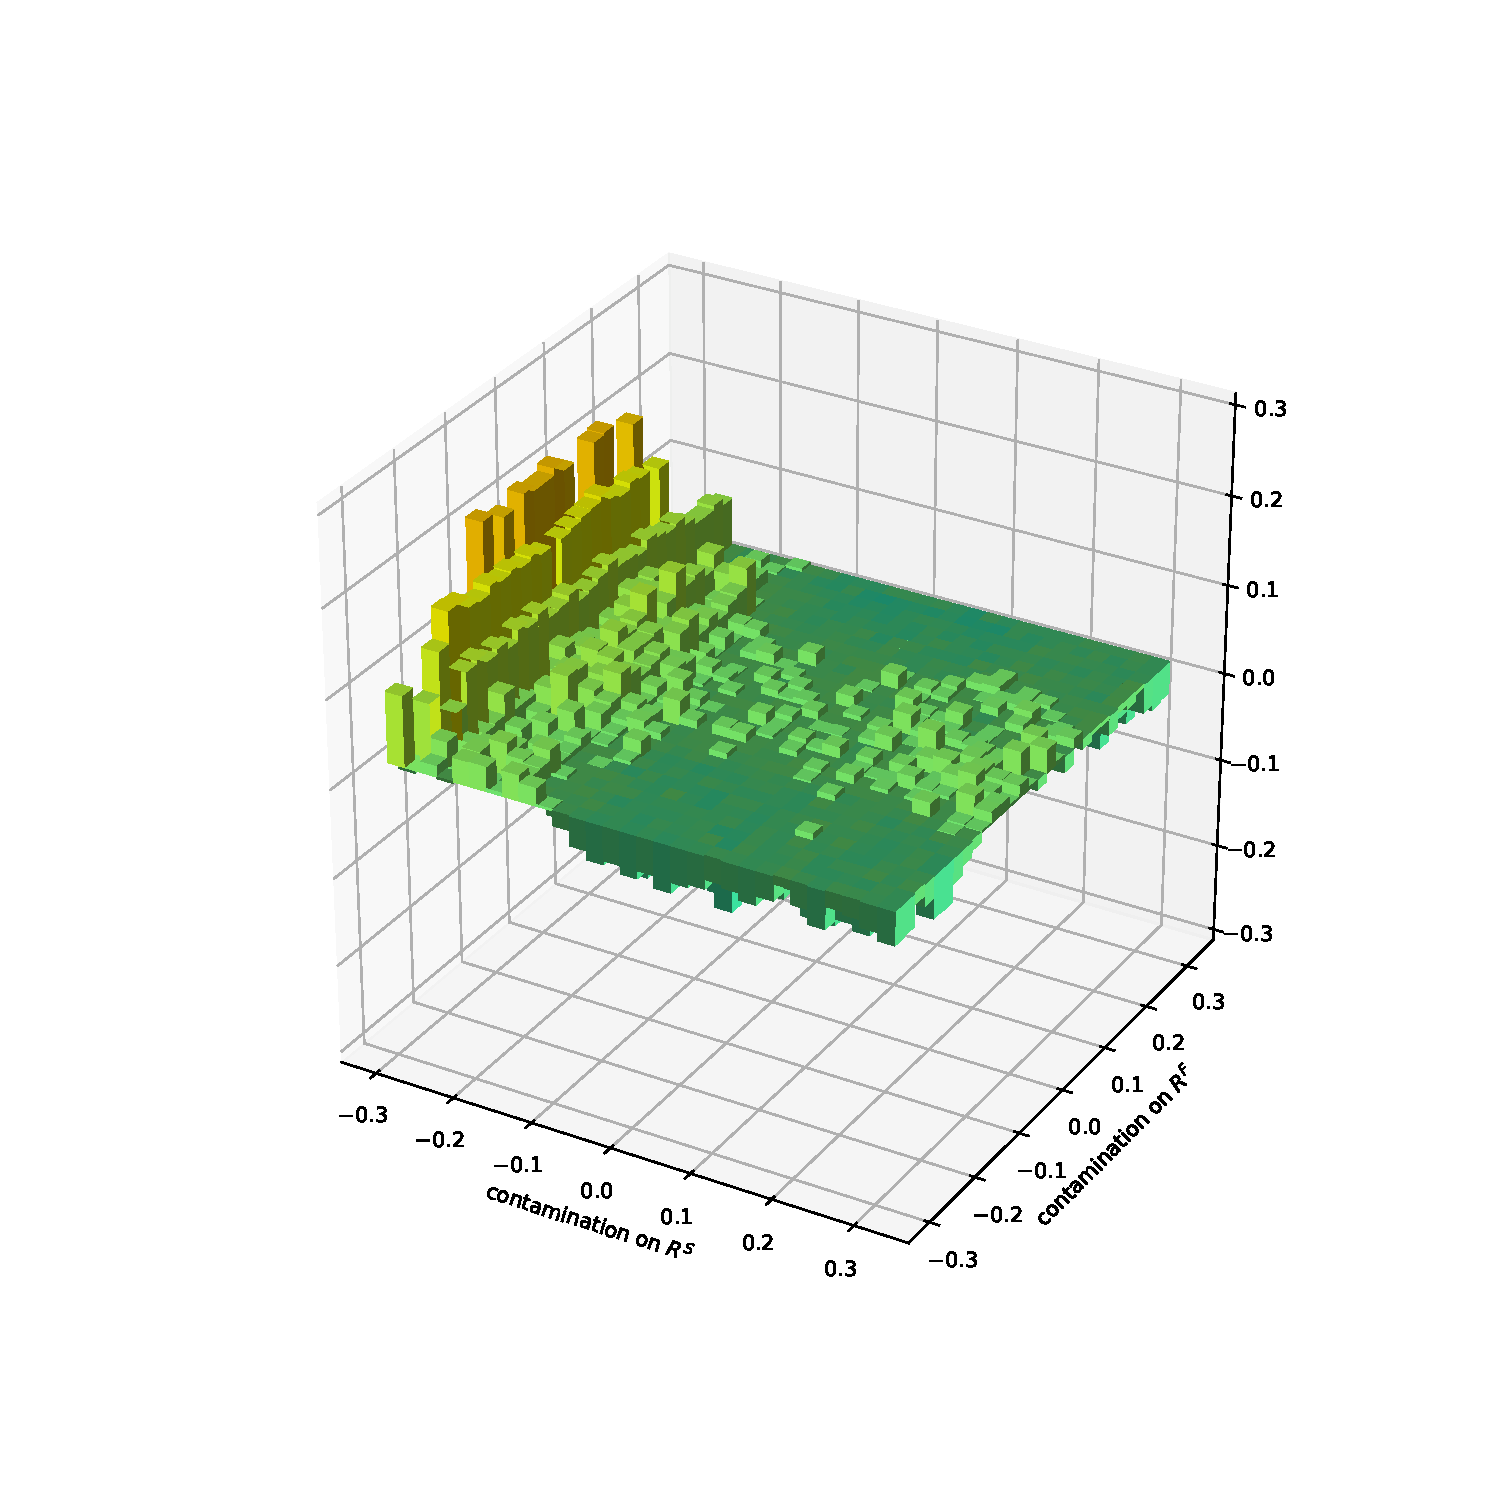
\includegraphics[height=5cm]{_pics/IF_plots/VaR1_t_copula_MLE.pdf} &
   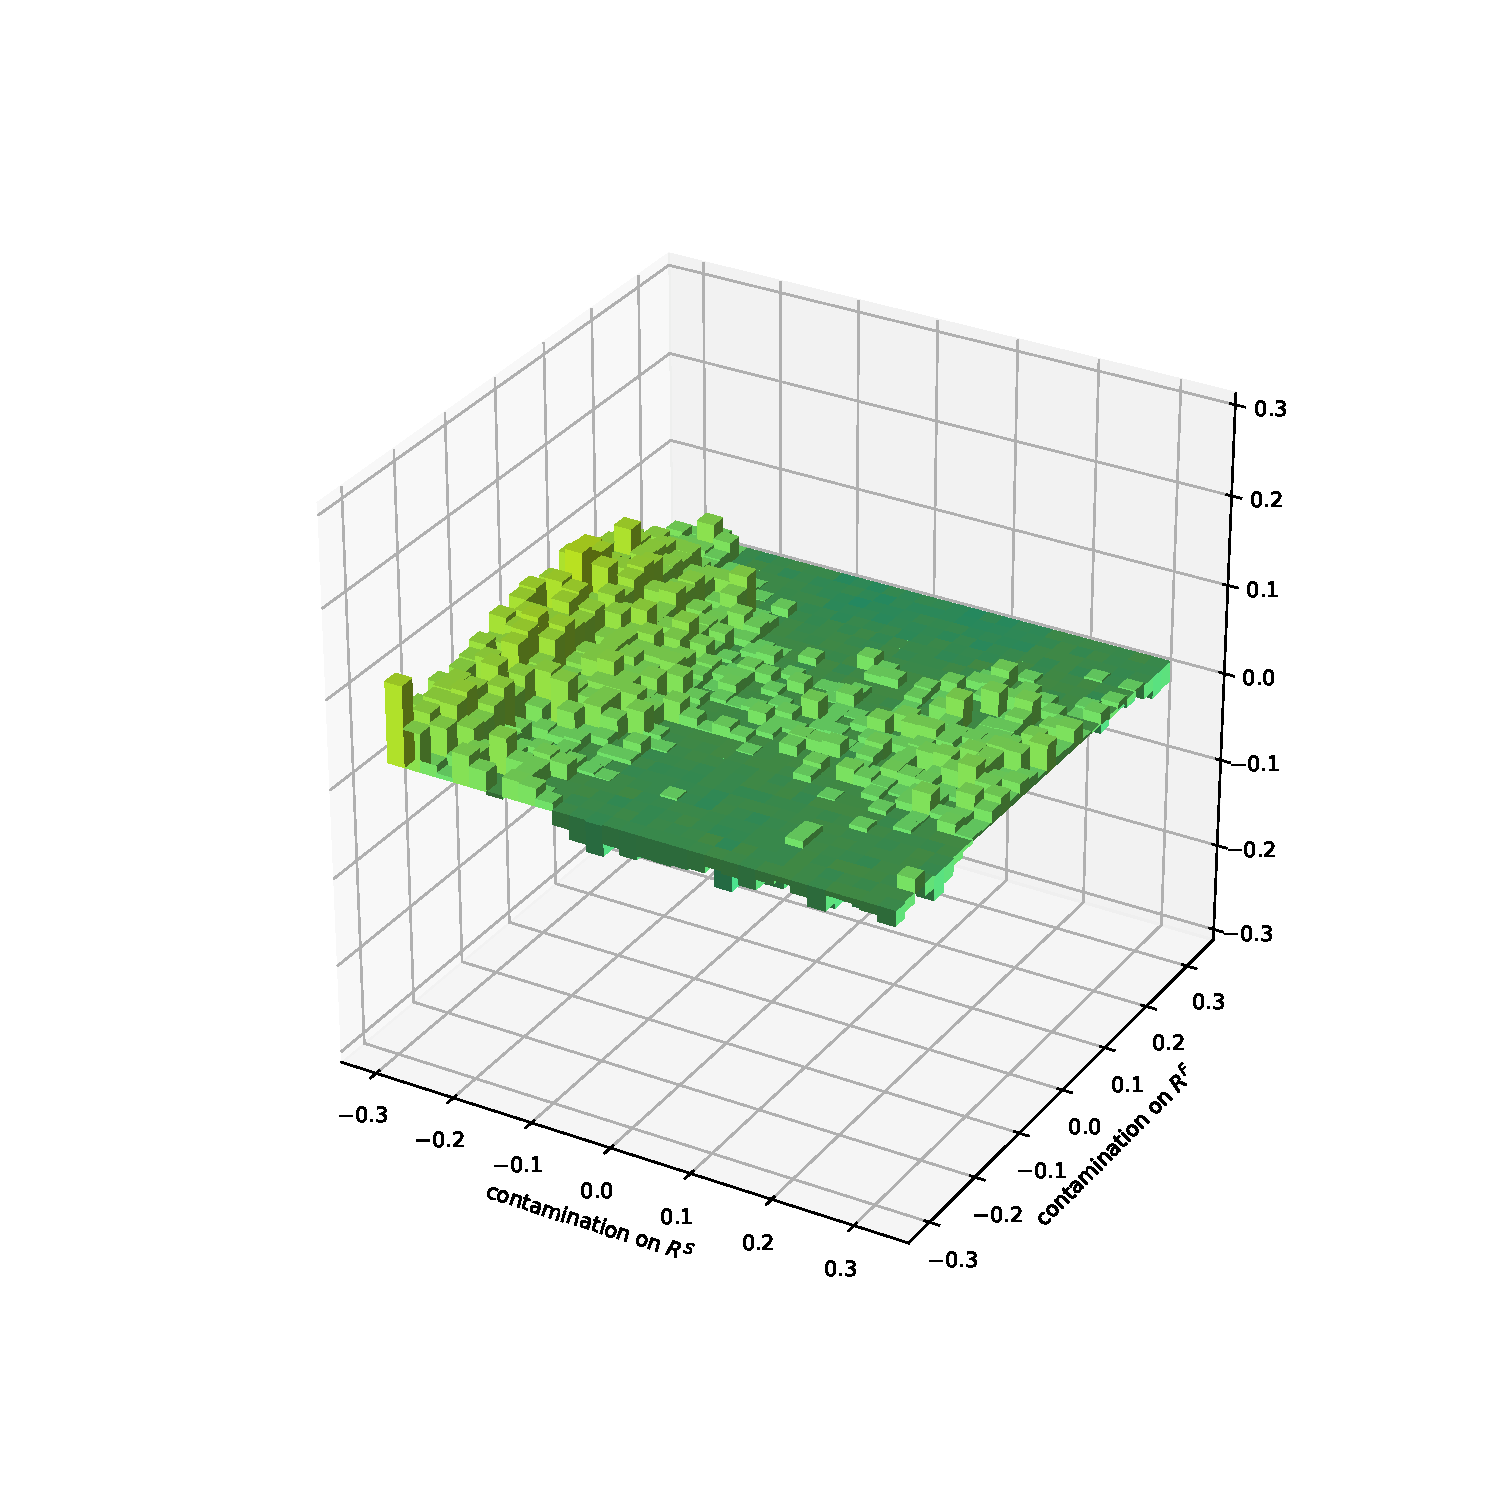
\includegraphics[height=5cm]{_pics/IF_plots/ES5_t_copula_MLE.pdf} &
   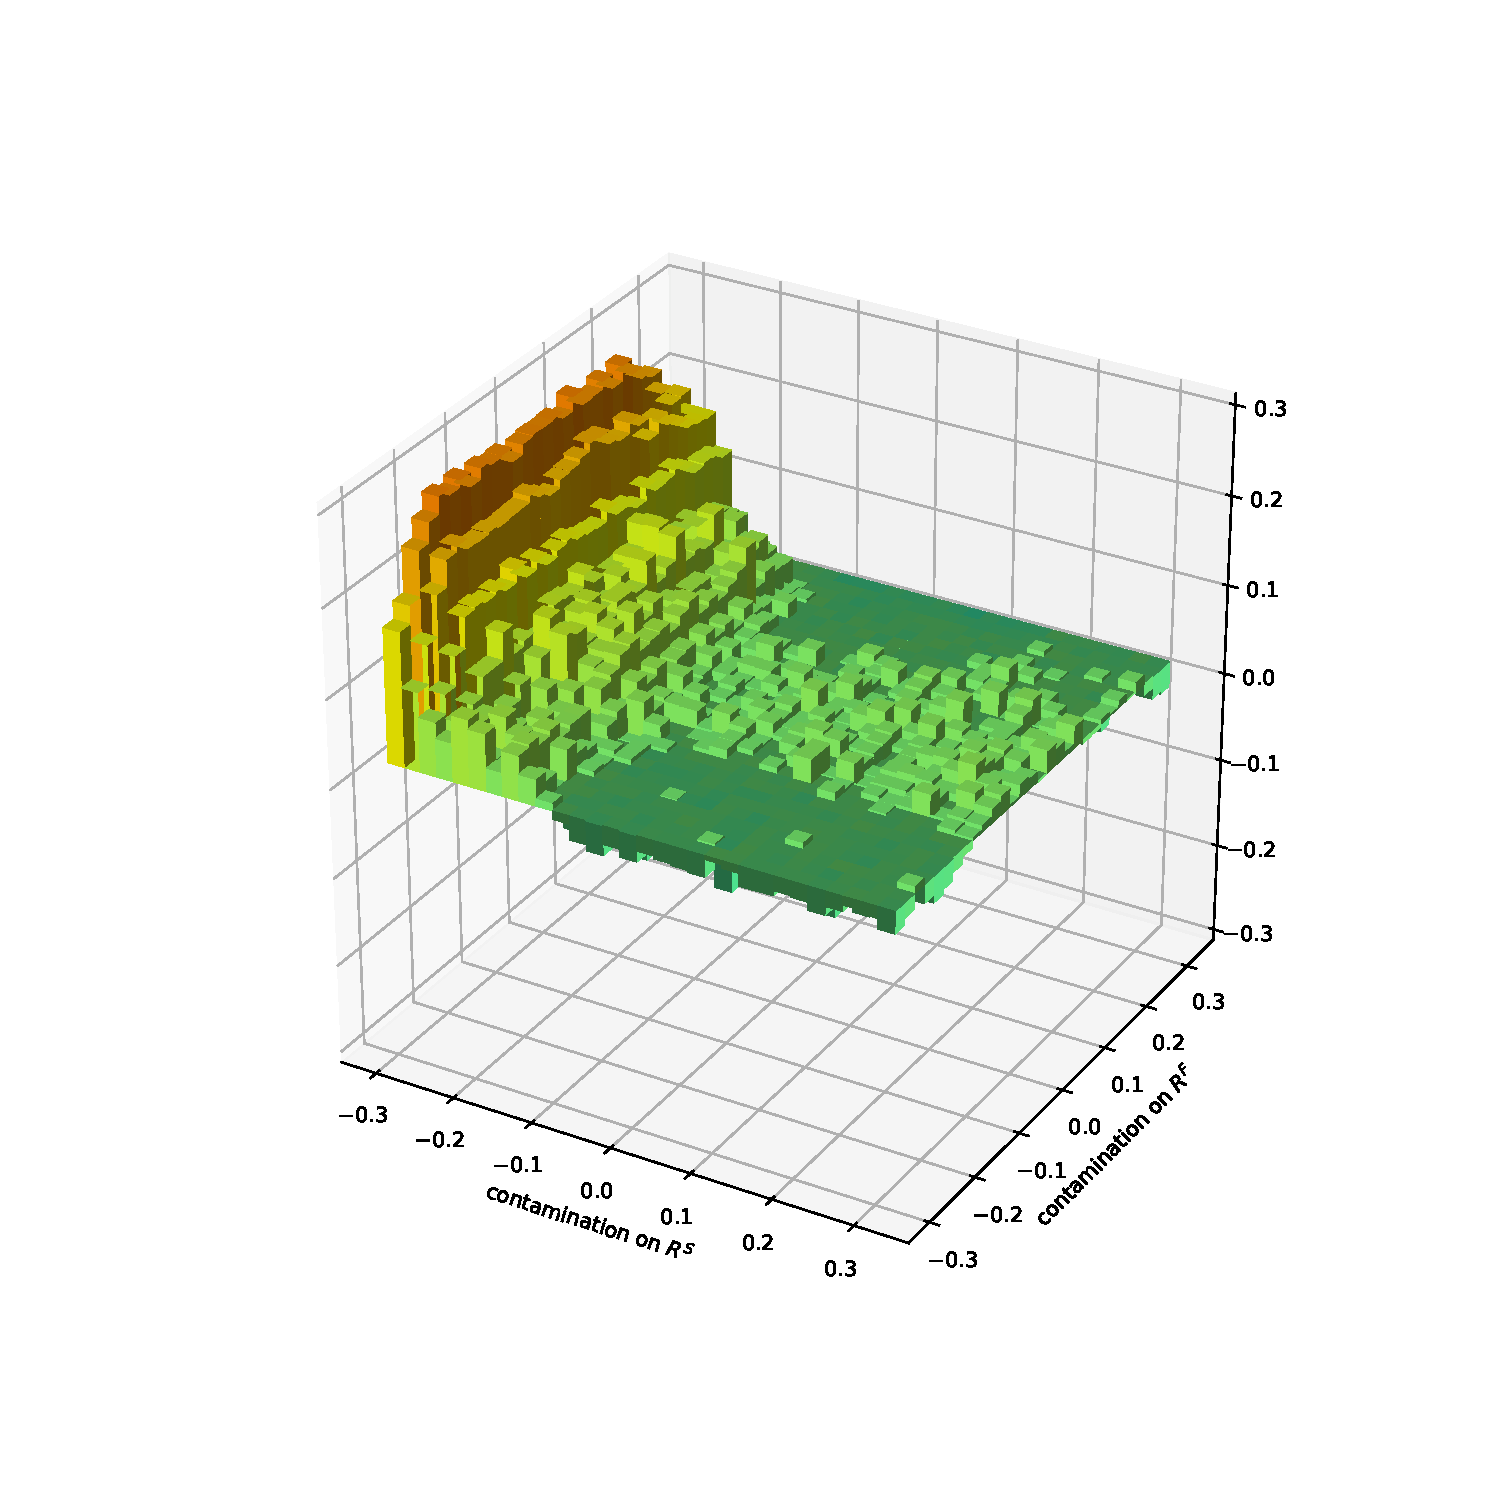
\includegraphics[height=5cm]{_pics/IF_plots/ES1_t_copula_MLE.pdf}
   \end{tabular}
   \caption{Influence functions (IF) of $h^*$ using $t$ copula copula estimated by MLE. From left to right, top to bottem, the plots are
   IF of using $\text{Var}$, $\text{ERM}_{10}$, $\text{VaR}_{0.95}$, $\text{VaR}_{0.99}$, $\text{ES}_{0.95}$, and $\text{ES}_{0.99}$ respectively.
   \href{http://www.quantlet.com/}{
\includegraphics[width=20pt]{_pics/qletlogo_tr.png}}}
   \label{fig:IFs}
\end{figure}





%We measure the stability of $h^*$ by sum of absolute change
%\begin{align}
%    \sum_{t=1}^T|h_t - h_{t-1}|.
%    \end{align}
%
%Adjustment of portfolio weights induces price slippage (ref) and transaction cost.
%From figure \ref{SAD} we know the NIG factor copula with variance as risk reduction objective generates the smallest
%sum of absolute change in OHR.
%
%\begin{figure}[!th]
%   \centering
%   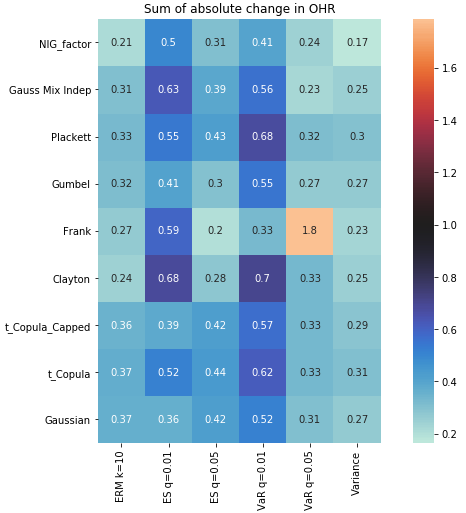
\includegraphics[width=\textwidth]{_pics/Sum of absolute change in OHR.png}
%   \caption{Sum of Absolute Change in OHR.
%   \href{http://www.quantlet.com/}{
\includegraphics[width=20pt]{_pics/qletlogo_tr.png}}}
%   \label{fig:SAD}
%\end{figure}

%%\usepackage{fontspec}
%\newcommand{\smallest}[1]{\textcolor{Maroon}{\textbf{#1}}}

\begin{table}
\begin{tabular}{lrrrrrr}
\toprule
{} &  ERM k=10 &    ES 99\% &    ES 95\% &   VaR 99\% &   VaR 95\% &  Variance \\
\midrule
Gaussian        &  0.019985 &  0.020802 &  0.020061 &  0.020230 &  0.019983 &  \color{blue}0.019757 \\
t\_Copula        &  0.020097 &  0.021698 &  0.020381 &  0.020966 &  0.020071 &  \color{blue}0.019890 \\
t\_Copula\_Capped &  0.020048 &  0.021018 &  0.020202 &  0.020554 &  0.020059 &  \color{blue}0.019792 \\
Clayton         &  0.019519 &  0.021341 &  0.019789 &  0.021045 &  \color{blue}0.019389 &  0.019675 \\
Frank           &  0.029234 &  0.026240 &  0.030770 &  0.029157 &  \color{blue}0.023085 &  0.025928 \\
Gumbel          &  0.020014 &  0.021411 &  0.020511 &  0.021643 &  \color{blue}0.019557 &  0.019757 \\
Plackett        &  0.020010 &  0.021531 &  0.020363 &  0.020870 &  \color{blue}0.019755 &  0.019909 \\
Gauss Mix Indep &  0.019949 &  0.025390 &  0.020454 &  0.023283 &  \color{blue}0.019667 &  0.020006 \\
NIG\_factor      &  \color{blue}0.019720 &  0.023425 &  0.020706 &  0.022039 &  0.019950 &  0.019999 \\
\bottomrule
\end{tabular}
\caption{Exponential Risk Measure $k=10$}
\end{table}

\begin{table}
\begin{tabular}{lrrrrrr}
\toprule
{} &  ERM k=10 &    ES 99\% &    ES 95\% &   VaR 99\% &   VaR 95\% &  Variance \\
\midrule
Gaussian        &  0.061084 &  0.062405 &  0.061201 &  0.062148 &  0.061712 &  \color{blue}0.059310 \\
t\_Copula        &  0.062148 &  0.068702 &  0.063339 &  0.063964 &  0.062067 & \color{blue}0.060735 \\
t\_Copula\_Capped &  0.061623 &  0.064114 &  0.062198 &  0.062466 &  0.062072 & \color{blue}0.059676 \\
Clayton         &  0.058495 &  0.069910 &  0.060812 &  0.064595 &  \color{blue}0.055962 &  0.058318 \\
Frank           &  0.104185 &  0.096795 &  0.108713 &  0.105070 &  \color{blue}0.068457 &  0.091321 \\
Gumbel          &  0.056513 &  0.059574 &  0.056035 &  0.058162 &  \color{blue}0.055492 &  0.059525 \\
Plackett        &  0.061167 &  0.068027 &  0.063426 &  0.064563 &  \color{blue}0.058491 &  0.061017 \\
Gauss Mix Indep &  0.061157 &  0.088023 &  0.063900 &  0.073316 &  \color{blue}0.057007 &  0.063081 \\
NIG\_factor      &  \color{blue}0.060878 &  0.078959 &  0.065270 &  0.070919 &  0.062097 &  0.062848 \\
\bottomrule
\end{tabular}
\caption{ES 99\%}
\end{table}

\begin{table}
\begin{tabular}{lrrrrrr}
\toprule
{} &  ERM k=10 &    ES 99\% &    ES 95\% &   VaR 99\% &   VaR 95\% &  Variance \\
\midrule
Gaussian        &  0.034488 &  0.035237 &  0.034548 &  0.035123 &  0.034838 &  \color{blue}0.034248 \\
t\_Copula        &  0.034777 &  0.037100 &  0.035234 &  0.035634 &  0.035055 &  \color{blue}0.034494 \\
t\_Copula\_Capped &  0.034647 &  0.035679 &  0.034862 &  0.035282 &  0.034937 &  \color{blue}0.034322 \\
Clayton         &  0.033714 &  0.037282 &  0.034230 &  0.036089 &  \color{blue}0.033445 &  0.034046 \\
Frank           &  0.053661 &  0.047849 &  0.056299 &  0.053409 &  \color{blue}0.037638 &  0.046953 \\
Gumbel          &  0.034028 &  0.035965 &  0.034528 &  0.036353 &  \color{blue}0.033568 &  0.034293 \\
Plackett        &  0.034592 &  0.036831 &  0.035316 &  0.035752 &  \color{blue}0.034186 &  0.034558 \\
Gauss Mix Indep &  0.034439 &  0.045160 &  0.035120 &  0.040027 &  \color{blue}0.033756 &  0.034478 \\
NIG\_factor      &  \color{blue}0.033882 &  0.041001 &  0.035677 &  0.037975 &  0.034656 &  0.034453 \\
\bottomrule
\end{tabular}
\caption{ES 95\%}
\end{table}

\begin{table}
\begin{tabular}{lrrrrrr}
\toprule
{} &  ERM k=10 &    ES 99\% &    ES 95\% &   VaR 99\% &   VaR 95\% &  Variance \\
\midrule
Gaussian        &  \color{blue}0.041327 &  0.044416 &  0.041943 &  0.043399 &  0.042275 &  0.041981 \\
t\_Copula        &  \color{blue}0.041450 &  0.044830 &  0.042806 &  0.043789 &  0.041693 &  0.041969 \\
t\_Copula\_Capped &  \color{blue}0.041498 &  0.044169 &  0.042411 &  0.044051 &  0.042018 &  0.042056 \\
Clayton         &  \color{blue}0.040022 &  0.044523 &  0.042878 &  0.044215 &  0.040913 &  0.041943 \\
Frank           &  0.076644 &  0.055387 &  0.081273 &  0.073433 &  \color{blue}0.046177 &  0.061056 \\
Gumbel          &  0.042079 &  0.042139 &  0.042187 &  0.045340 &  \color{blue}0.040523 &  0.041937 \\
Plackett        &  \color{blue}0.041013 &  0.044971 &  0.042370 &  0.042995 &  0.041574 &  0.041731 \\
Gauss Mix Indep &  0.040998 &  0.048017 &  0.043249 &  0.044518 &  \color{blue}0.040749 &  0.043386 \\
NIG\_factor      &  \color{blue}0.040457 &  0.047201 &  0.043925 &  0.044230 &  0.043240 &  0.043138 \\
\bottomrule
\end{tabular}
\caption{VaR 99\%}
\end{table}

\begin{table}
\begin{tabular}{lrrrrrr}
\toprule
{} &  ERM k=10 &    ES 99\% &    ES 95\% &   VaR 99\% &   VaR 95\% &  Variance \\
\midrule
Gaussian        &  0.020385 &  0.020315 &  0.020143 &  0.020412 &  0.020121 &  \color{blue}0.019579 \\
t\_Copula        &  0.020547 &  0.020428 &  0.020661 &  0.020611 &  0.020370 &  \color{blue}0.019820 \\
t\_Copula\_Capped &  0.020525 &  0.020544 &  0.020503 &  0.020486 &  0.020224 &  \color{blue}0.019656 \\
Clayton         &  0.019702 &  0.021042 &  0.020143 &  0.020640 &  0.019990 &  \color{blue}0.019700 \\
Frank           &  0.026372 &  0.023529 &  0.027105 &  0.026212 &  \color{blue}0.023389 &  0.023594 \\
Gumbel          &  0.019781 &  0.021311 &  0.020716 &  0.020421 &  \color{blue}0.019077 &  0.019541 \\
Plackett        &  0.020459 &  0.020257 &  0.020589 &  0.020100 &  0.020237 &  \color{blue}0.020047 \\
Gauss Mix Indep &  0.020482 &  0.024753 &  0.020304 &  0.024158 &  \color{blue}0.019944 &  0.020723 \\
NIG\_factor      &  \color{blue}0.019923 &  0.023784 &  0.021009 &  0.022172 &  0.019980 &  0.020670 \\
\bottomrule
\end{tabular}
\caption{VaR 95\%}
\end{table}

\begin{table}
\begin{tabular}{lrrrrrr}
\toprule
{} &  ERM k=10 &    ES 99\% &    ES 95\% &   VaR 99\% &   VaR 95\% &  Variance \\
\midrule
Gaussian        &  0.014387 &  0.014380 &  0.014360 &  0.014530 &  0.014670 &  \color{blue}0.014294 \\
t\_Copula        &  0.014378 &  0.014626 &  0.014343 &  0.014385 &  0.014627 &  \color{blue}0.014306 \\
t\_Copula\_Capped &  0.014375 &  0.014418 &  0.014332 &  0.014430 &  0.014643 &  \color{blue}0.014290 \\
Clayton         &  0.014306 &  0.014870 &  0.014332 &  0.014532 &  0.014493 &  \color{blue}0.014267 \\
Frank           &  0.021495 &  0.018982 &  0.022736 &  0.021476 &  \color{blue}0.018142 &  0.018897 \\
Gumbel          &  0.014618 &  0.014971 &  0.014878 &  0.015438 &  0.014622 &  \color{blue}0.014321 \\
Plackett        &  0.014444 &  0.014560 &  0.014424 &  0.014423 &  0.014596 &  \color{blue}0.014353 \\
Gauss Mix Indep &  0.014404 &  0.017404 &  \color{blue}0.014341 &  0.015671 &  0.014453 &  0.014408 \\
NIG\_factor      &  \color{blue}0.014362 &  0.015841 &  0.014484 &  0.015043 &  0.014474 &  0.014415 \\
\bottomrule
\end{tabular}
\caption{Standard Deviation}
\end{table}